\documentclass[a4paper,12pt]{article}

\usepackage{graphicx}
\usepackage[usenames,dvipsnames]{xcolor}
\usepackage{tcolorbox}
\usepackage{tabularx}
\usepackage{array}
\usepackage{colortbl}
\tcbuselibrary{skins}
\usepackage{tablefootnote}
\usepackage[a4paper, total={6.5in, 8in}]{geometry}
\usepackage[backend=biber,style=numeric,citestyle=authortitle-ibid]{biblatex}
\usepackage{qrcode}
\usepackage{environ}
\usepackage{xcolor}
\usepackage[tikz]{bclogo}
\usepackage{tikz}
\usetikzlibrary{calc}
\usepackage[colorlinks=true,linkcolor=blue]{hyperref}
\usepackage[utf8]{inputenc}
\usepackage{tabularx}

% Steps
\usepackage{enumitem}
\newlist{steps}{enumerate}{1}
\setlist[steps, 1]{label = Step \arabic*:}

\newcolumntype{Y}{>{\raggedleft\arraybackslash}X}

\tcbset{tab1/.style={fonttitle=\bfseries\large,fontupper=\normalsize\sffamily,
colback=yellow!10!white,colframe=red!75!black,colbacktitle=Salmon!40!white,
coltitle=black,center title,freelance,frame code={
\foreach \n in {north east,north west,south east,south west}
{\path [fill=red!75!black] (interior.\n) circle (3mm); };},}}

\tcbset{tab2/.style={enhanced,fonttitle=\bfseries,fontupper=\normalsize\sffamily,
colback=yellow!10!white,colframe=red!50!black,colbacktitle=Salmon!40!white,
coltitle=black,center title}}

\newcounter{stepcounter}

\addbibresource{cite.bib} % include citation file

\begin{document}
\begin{titlepage}
    \centering 
    \vfill
    
\includegraphics[width=10cm]{ilri_logo.png}
    \vfill 
    {\bfseries\Large
        USER GUIDE\\
        FOR\\
        FEED FORMULATION APPLICATION\\
        \vskip2cm
    }   
    
    \vfill 
    \vfill 
    \vspace{50pt}
    \textbf{A comprehensive user manual for Feed Formulation App\\
			Addis Ababa, ETHIOPIA\\
			Version 1.0\\
			26/12/2023
		}
    
    \vfill
\end{titlepage}

\newpage

\tableofcontents
\newpage

\pagenumbering{arabic}

\section{Legend}
\begin{tcolorbox}[tab2,tabularx={X|Y|Y|Y|Y}]
\textbf{Name} & \textbf{Abbreviation} & \textbf{Unit}  & \textbf{Description} \\\hline
Dry matter & DM & \% &  The dry matter or dry weight is a measure of the mass of a completely dried substance.\footcite{enwiki:1178208071} \\\hline

Metabolizable Energy   & ME & kcal/kg 	&  \\\hline

Crude protein   	& CP	& \% 		&  \\\hline
Lysine   & Lys 		& \% 	&	\\\hline
Meth. +cystine   	& m+c 	& \% 		&  \\\hline
Methionine   		& Met 	& \% 		&  \\\hline
Ether extract   		& EE 	& \% 		&  \\\hline
Crude fiber   		& CF 	& \% 		&  \\\hline
Calcium & Ca 	& \% 		&  \\\hline
Phosphorus   		& P 	& \% 		&  \\\hline
\end{tcolorbox}

\section{Glossary}
\begin{tabular}{p{8cm}p{11cm}}
Ration &  \\
\\
Formulation &  \\
\\
Formula &  \\
\\
Grid Formulation &  \\
\\
Ingredients &  \\
\\
Ingredient Group &  \\
\\
Ingredient Composition &  \\
\\
Nutrient Group &  \\
\\
Nutrients &  \\
\\
Requirements &  \\
\\
Requirement Compostion &  \\
\\
Requirement Boundires & (Min \& Max)  \\
\\

\\

\end{tabular}

\newpage
\section{Introduction}

This guide outlines the TPGS websites' capabilities and walks you through how you can use the application.

Acess the webiste using either the below url or QR code.


\NewEnviron{myremark}[1]
  {\par\medskip\noindent
  \begin{tikzpicture}
    \node[inner sep=0pt] (box) {\parbox[t]{.99\textwidth}{%
      \begin{minipage}{.3\textwidth}
      \centering\tikz[scale=5]\node[scale=3,rotate=30]{\bclampe};
      \end{minipage}%
      \begin{minipage}{.65\textwidth}
      \textbf{#1}\par\smallskip
      \BODY
      \end{minipage}\hfill}%
    };
    \draw[red!75!black,line width=3pt] 
      ( $ (box.north east) + (-5pt,3pt) $ ) -- ( $ (box.north east) + (0,3pt) $ ) -- ( $ (box.south east) + (0,-3pt) $ ) -- + (-5pt,0);
    \draw[red!75!black,line width=3pt] 
      ( $ (box.north west) + (5pt,3pt) $ ) -- ( $ (box.north west) + (0,3pt) $ ) -- ( $ (box.south west) + (0,-3pt) $ ) -- + (5pt,0);
  \end{tikzpicture}\par\medskip%
}

\begin{myremark}{To Access The App}\label{visite_site}
\vspace{10px}
Scan the QR Code or go to: \href{https://tpgs.ilri.org/}{https://tpgs.ilri.org/}

\vspace{20px}

\quad
\qrcode[height=1in]{https://tpgs.ilri.org/?qrcode=true}
\end{myremark}

\newpage

\section{Feed Formulation in Poultry Farming}
Feed formulation is crucial in poultry farming, as it directly impacts chicken health,
growth, and productivity. Properly formulated feed ensures that chickens receive the
right balance of essential nutrients—proteins, carbohydrates, fats, vitamins, and
minerals—which are necessary for optimal growth, egg production, and overall health. A
well-balanced diet not only enhances growth and reproduction but also helps reduce
disease risk, improves feed conversion rates, and lowers production costs. However,
feed formulation is not a one-size-fits-all solution. It must account for factors such as the
chicken's age, breed, production purpose (meat, egg, or breeding), and environmental
conditions. Achieving the right balance requires knowledge of nutritional needs,
available feed ingredients, and local farming conditions.

\newpage
\section{Poultry Nutrients and Their Functions}
Poultry feed contains several essential nutrients, each playing a vital role in chicken
health, growth, and productivity. These nutrients include:

\paragraph{Proteins and Amino Acids}
\begin{description}
	\item[Function:] Proteins are the building blocks for growth, muscle
development, tissue repair, and egg production. Amino acids like \textbf{Lysine}
and \textbf{Methionine} are essential for optimal growth.
	\item[Sources:] Soybean meal, fish meal, alfalfa.
\end{description}


\paragraph{Carbohydrates}
\begin{description}
	\item[Function:] Provide the primary energy source for chickens, supporting
heat production, activity, and metabolism.
	\item[Sources:] Corn, wheat, rice, barley.
\end{description}

\paragraph{Fats (Lipids)}
\begin{description}
	\item[Function:] Provide concentrated energy, assist in fat-soluble vitamin
absorption, and support cell structure.
	\item[Sources:] Vegetable oils, fish oils, seeds.
\end{description}

\paragraph{Vitamins}
\begin{description}
	\item[Function:] Support immune health, metabolism, and tissue development.
Key vitamins include \textbf{A, D, E,} and B-vitamins (B12, niacin, folic acid).
	\item[Sources:] Vegetables, fruits, liver, fish meal, yeast.
\end{description}

\paragraph{Minerals}
\begin{description}
	\item[Function:] Essential for bone development, enzyme function, and
electrolyte balance. \textbf{Calcium} and \textbf{Phosphorus} are critical for bone health
and eggshell formation.
	\item[Sources:] Limestone, dicalcium phosphate, salt, trace minerals.
\end{description}

\paragraph{Water}
\begin{description}
	\item[Function:] Vital for digestion, nutrient absorption, temperature regulation,
and overall cellular function.
	\item[Sources:] Clean, fresh water is essential for hydration.
\end{description}

\paragraph{Fiber}
\begin{description}
	\item[Function:] Aids in digestion and gut health, supporting motility and proper
droppings formation.
	\item[Sources:] Wheat bran, vegetable matter, rice hulls.
\end{description}

\paragraph{Antioxidants}
\begin{description}
	\item[Function:] Protect cells from oxidative damage and support immune
function. \textbf{Vitamin E} and \textbf{Selenium} are key antioxidants.
	\item[Sources:] Vegetable oils, selenium-enriched grains.
\end{description}

\paragraph{Enzymes}
\begin{description}
	\item[Function:] Improve feed efficiency by aiding in digestion and nutrient
absorption.
	\item[Sources:] Naturally occurring in feed or supplemented.
\end{description}


\subsubsection{Nutrient Balancing}
For optimal poultry health and productivity, nutrient balance is key. For example:

\begin{itemize}
	\item An imbalance of calcium and phosphorus can affect bone health or eggshell
quality.
	\item A proper balance between protein and energy is crucial to support growth,
laying, or meat production, depending on the bird's purpose.
\end{itemize}

\newpage
\section{The Role of Feed Formulation Apps}
Advancements in technology have simplified feed formulation through user-friendly
apps. These apps make the complex process of creating a balanced poultry diet
accessible to both smallholder farmers and large-scale producers. The apps offer
features that streamline the formulation process, such as:

\begin{description}
	\item[Simple Interface:] Intuitive design for users with varying technical expertise,
allowing them to input chicken details (age, weight, goals) and get customized
feed recommendations.
	\item[Ingredient Database:] Comprehensive databases that include local and
international feed ingredients, enabling users to create balanced rations with
familiar or locally available resources.
	\item[Nutrient Balancing:] Automatically adjusts feed formulations to meet specific
nutritional requirements, ensuring proper growth, egg production, or other
specific outcomes.
	\item[Cost Optimization:] Users can input local feed prices, helping them create cost-
effective formulations without compromising on nutritional quality.
	\item[Sustainability and Local Resources:] Apps support sustainable practices by
recommending locally available feed resources, reducing reliance on imported
ingredients, and minimizing waste.
	\item[Data-Driven Insights:] Some apps provide analytical tools to track feed
efficiency, growth rates, and other performance metrics, enabling informed
decision-making.
\end{description}

\subsection{Flexibility and Sustainability in Feed Formulation}
Feed formulation apps allow flexibility in using locally available feed ingredients,
especially in regions where commercial feed is expensive or inaccessible. These apps
help farmers utilize alternative feed sources, such as grains, legumes, agricultural by-
products, and even insects, to develop affordable and sustainable feeding strategies.
Locally sourced ingredients are often cheaper and help reduce dependency on external
suppliers, contributing to the local economy.


Furthermore, the use of agro-industrial by-products (e.g., rice bran, cassava leaves) is
encouraged, fostering a circular agricultural economy. These practices not only lower
feed costs but also support long-term sustainability in poultry farming by reducing
waste.

\subsection{Affordable and Sustainable Feeding Solutions}
Feed formulation apps support affordable and sustainable feeding solutions by:

\begin{description}
	\item[Optimizing Feed Costs:] Ensuring efficient use of local ingredients and
minimizing waste.
	\item[Preventing Over- or Under-Feeding:] Correctly balancing the diet helps avoid
unnecessary expenses or health issues related to improper feeding.
	\item[Supporting Sustainability:] By promoting locally available ingredients and
reducing reliance on costly commercial feed, apps help ensure the sustainability
of poultry farming in the long term.
\end{description}

\newpage
\section{Protein Requirements in Poultry Nutrition}
Meeting the amino acid requirements of poultry through balanced protein sources is
essential for optimal growth, productivity, and product quality. By carefully selecting and
balancing protein ingredients, poultry producers can formulate diets that support both
economic and nutritional efficiency.

\subsection{Protein components}

\paragraph{Essential Amino Acids:}
\begin{itemize}
	\item Poultry cannot synthesize essential amino acids, which include
methionine, lysine, threonine, and tryptophan, among others. Therefore,
these amino acids must be supplied through dietary protein sources.
	\item The \textbf{quality of a protein} source is often judged by its amino acid profile,
specifically whether it contains adequate amounts of these essential
amino acids. High-quality protein sources will meet poultry’s requirements
for essential amino acids, which are critical for muscle growth, feathering,
and production performance.
\end{itemize}

\paragraph{Multiple Protein Sources:}
\begin{itemize}
	\item \textbf{No single feed ingredient} provides all essential amino acids in the
necessary proportions for poultry. Consequently, formulating a balanced
poultry ration requires combining multiple protein sources. This ensures
the diet includes a well-rounded profile of amino acids.
	\item Typically, poultry diets are formulated with a mix of plant-based proteins
(like soybean meal, corn gluten meal, or canola meal) and, if permitted,
animal-based proteins (such as fish meal or meat and bone meal).
\end{itemize}

\paragraph{Limiting Amino Acids:}
\begin{itemize}
	\item \textbf{Methionine and lysine} are known as the “limiting amino acids” in poultry
nutrition. They are often present in lower quantities in most feed ingredients relative to the birds’ requirements, which can restrict growth if not supplemented adequately.
	\item Synthetic forms of these amino acids, such as \textbf{DL-Methionine} and \textbf{L-
Lysine}, are commonly added to poultry feed to meet these requirements.
Supplementing these amino acids improves protein utilization in the diet
and reduces the need for excess dietary protein.
\end{itemize}

\paragraph{Anti-Nutritional Factors (ANFs):}
\begin{itemize}
	\item Poultry, particularly chickens, are sensitive to \textbf{anti-nutritional factors}
(ANFs) that are present in some plant-based feed ingredients. ANFs, such
as trypsin inhibitors in raw soybeans or tannins in some legumes, can
interfere with protein digestion and amino acid absorption.
	\item  Processing methods, like heat treatment, are used to reduce ANFs in
ingredients like soybean meal, making them safer and more digestible for
poultry.
\end{itemize}

\paragraph{Fish Meal Consideration:}
\begin{itemize}
	\item \textbf{Fish meal} is a rich source of protein and essential amino acids,
particularly lysine and methionine. However, when included at levels
above \textbf{5\% of the total diet}, it can impart a fishy taste to poultry meat and
eggs.
	\item For this reason, fish meal is usually limited in poultry diets unless the birds
are not raised for human consumption or taste alteration is not a concern.
\end{itemize}

\subsection{Common Protein Sources in Poultry Diets}
\begin{description}
	\item[Soybean Meal:] A high-quality plant protein with a good balance of essential
amino acids, widely used in poultry diets.
	\item[Corn Gluten Meal:] Provides protein and energy, but is low in lysine, so it needs
to be balanced with other ingredients.
	\item[Fish Meal:] High in lysine and methionine but limited due to its potential effect on
meat and egg flavor.
	\item[Meat and Bone Meal:] Provides animal protein and minerals like calcium and
phosphorus but is restricted in some countries due to regulatory concerns.
	\item[Synthetic Amino Acids:] DL-Methionine and L-Lysine are often supplemented to
ensure the diet meets the birds’ requirements.
\end{description}

\newpage

\section{Fatty acid requirement in poultry}
\subsection{Fatty acid considerations}

\begin{description}
	\item[Essential Fatty Acid Requirement]:
		\begin{itemize}
			\item Linoleic acid is classified as an essential fatty acid for poultry because birds lack the necessary enzymes to synthesize it from other nutrients. This means it must
be supplied through the diet. Essential fatty acids are crucial for maintaining
cellular membrane integrity, immune function, and skin health in poultry.
			\item Studies show that linoleic acid is particularly important for growth, feathering, and reproductive health in poultry. Deficiency in linoleic acid can lead to poor growth
rates, reduced egg production, and impaired egg hatchability in breeders.
		\end{itemize}
		
	\item[Dietary Role of Fat in Poultry Nutrition]:
		\begin{itemize}
			\item Fats or oils are added to poultry diets not only as a concentrated energy source but also to improve nutrient absorption, particularly for fat-soluble vitamins (A, D,
E, and K). These vitamins are essential for various physiological functions,
including bone development, antioxidant defense, immune function, and
reproduction.
			\item Fats help reduce the dustiness of feed, making it more palatable and less likely to cause respiratory irritation. Improved palatability also encourages feed intake,
supporting growth and productivity.
		\end{itemize}
		
	\item[Antioxidants in Fat-Containing Poultry Diets]:
		\begin{itemize}
			\item When fats or oils are added to poultry diets, there is a risk of lipid oxidation, which can lead to rancidity. Rancid fats can reduce feed palatability and degrade
fat-soluble vitamins, impacting the bird's health and performance.
			\item Antioxidants such as ethoxyquin, BHT (butylated hydroxytoluene), and vitamin E are commonly included in fat-containing poultry feeds to prevent oxidation. By
preserving the stability of dietary fats, antioxidants help maintain the nutritional
quality of the feed.
		\end{itemize}
\end{description}

\newpage

\section{Mineral Requirements in Poultry Diets}
\subsection{Minerals considerations}
\begin{description}
	\item[Macrominerals vs. Microminerals]:
		\begin{itemize}
			\item Poultry require higher levels of \textbf{macrominerals} and lower levels of
\textbf{microminerals} to support essential physiological functions.
			\item \textbf{Macrominerals} include calcium (Ca), phosphorus (P), chloride (Cl), magnesium
(Mg), potassium (K), and sodium (Na). These minerals are needed in larger
amounts as they play crucial roles in skeletal development, electrolyte balance,
nerve function, and muscle contraction.
			\item \textbf{Microminerals} (or trace minerals) include copper (Cu), iodine (I), iron (Fe), manganese (Mn), selenium (Se), and zinc (Zn). Although required in smaller
quantities, microminerals are vital for enzyme function, immune response,
antioxidant defense, and thyroid function.
		\end{itemize}
		
	\item[Mineral Deficiency in Grains]:
		\begin{itemize}
			\item Grains, which are often a primary energy source in poultry diets, tend to be low in both macro- and microminerals. Consequently, poultry diets require
supplementation to ensure birds receive adequate mineral levels for optimal
growth, health, and productivity.
		\end{itemize}
\end{description}

\subsection{Common Sources of Macrominerals}
\begin{description}
	\item[Calcium (Ca):] Calcium is critical for bone health and eggshell formation in laying
hens. Common sources include limestone and oyster shell, both of which are
highly bioavailable forms of calcium. Limestone is often used in broiler diets,
while oyster shell is more common in layer diets for sustained calcium release.
	\item[Phosphorus (P):] Dicalcium phosphate is a primary source of both phosphorus
and calcium in poultry diets. Phosphorus works in tandem with calcium for bone
development and metabolic functions.
	\item[Other Macrominerals:] Sodium and chloride are often provided through salt
(NaCl), which maintains electrolyte balance, while potassium is naturally present
in some feed ingredients or provided through potassium chloride as needed.
\end{description}

\subsection{Mineral Premixes for Microminerals}
\begin{itemize}
	\item \textbf{Microminerals} are supplied in a\textbf{ mineral premix}, which is added to the feed in small amounts. The premix is carefully formulated to provide the necessary
levels of each trace mineral without risking toxicity. For example, zinc and
manganese are essential for bone and immune health, while selenium functions
as an antioxidant, protecting cells from oxidative damage.
\end{itemize}

\subsection{Categories of Vitamins in Poultry Nutrition}
\begin{itemize}
	\item Fat-Soluble Vitamins (A, D, E, and K):
	\begin{itemize}
		\item These vitamins are essential for various physiological functions:
			\begin{description}
				\item[Vitamin A:] Crucial for vision, immune function, and growth.
				\item[Vitamin D:] Important for calcium absorption, bone formation, and eggshell quality.
				\item[Vitamin E:] Acts as an antioxidant, protecting cells from oxidative damage, and supports immune function.
				\item[Vitamin K:] Needed for blood clotting and bone health.
			\end{description}
		\item Since these vitamins are stored in body fat, they need to be provided in
moderate, consistent amounts to prevent deficiency or toxicity.
	\end{itemize}
	
	\item \textbf{Water-Soluble Vitamins (Vitamin C and B Vitamins):}
		\begin{description}
			\item[Vitamin C:] Poultry can synthesize vitamin C, so it isn’t usually required in diets. However, it can be beneficial during periods of stress (e.g., heat stress) to
improve resilience and support immune function.
			\item[B Vitamins:] This group includes thiamine, riboflavin, niacin, pantothenic acid,pyridoxine, biotin, folic acid, and vitamin B12. B vitamins are essential for energy
metabolism, nerve function, and growth.
			\item These vitamins are not stored in the body to a great extent, so they need to be provided continuously in the diet.
		\end{description}
		
	\item \textbf{Endogenous and Exogenous Vitamin Sources:}
		\begin{itemize}
			\item While poultry can produce certain vitamins endogenously, particularly vitamin C and some B vitamins through microbial synthesis in the digestive tract, it’s often
insufficient to meet their complete nutritional needs.
			\item \textbf{Feed Ingredients as Vitamin Sources:} Some vitamins are naturally present in feed ingredients. For example, alfalfa meal and distillers' dried solubles contain B vitamins and may contribute to the overall vitamin content of the diet. However,
levels can vary significantly based on processing and storage conditions.
		\end{itemize}
		
	\item \textbf{Vitamin Premix for Consistency:}
	\begin{itemize}
		\item A \textbf{vitamin premix} is typically included in poultry diets to ensure consistent vitamin intake, compensating for the variability in vitamin content of natural feed
ingredients. Premixes are formulated to provide the optimal levels of vitamins
needed for growth, reproduction, and health.
	\end{itemize}
\end{itemize}

\newpage

\section{Common Poultry Feed Ingredients and Their Recommended Inclusion Levels}
Below is the list of common poultry feed ingredients, including their general inclusion rates and
safe limits for use in poultry feed formulations. The actual proportions can vary based on poultry
type (broilers, layers, breeders) and production stage (starter, grower, finisher). Note that
ingredient availability, nutrient composition, and cost can also influence ingredient usage. Safe
minimum and maximum ranges are essential for balancing nutrition and preventing toxicity or
health issues. Here's a comprehensive list of commonly used poultry feed ingredients, categorized into animal and plant protein sources, along with their safe minimum and maximum inclusion levels in feed formulation. I've also added additional details to aid in ration formulation.

\subsection{Animal Protein Sources}
Animal protein sources provide essential amino acids, vitamins, and minerals but must be
carefully monitored to avoid imbalances in nutrients and excessive levels of heavy metals.

\begin{table}[]
\begin{tabularx}{1\textwidth} { 
  | >{\raggedright\arraybackslash}X 
  | >{\centering\arraybackslash}X 
  | >{\centering\arraybackslash}X 
  | >{\centering\arraybackslash}X 
  | >{\raggedleft\arraybackslash}X | }
 
\hline
\textbf{Ingredient} & \textbf{Safe Minimum (\%)} & \textbf{Safe Maximum (\%)} & \textbf{Purpose}  & \textbf{Notes and Safe Usage} \\
\hline

Fish Meal & 2 & 10 & High-quality protein, omega-3 &  Ensure quality control to avoid spoilage and rancidity. High in phosphorus. \\
\hline

Meat and Bone Meal & 0 & 5 & Protein and calcium source & Provides phosphorus and
calcium but has variable protein
quality. Limit to avoid
imbalances in non-layers. \\
\hline

Blood Meal & 0 & 3 & Protein, high
lysine
content & Use with caution due to high
protein concentration. Limit to
avoid palatability issues. \\

\hline

Feather Meal & 0 & 5 & Protein,
primarily
keratin & High in cysteine but low in
digestibility unless hydrolyzed. \\
\hline

Poultry By-
product Meal & 0 & 10 & Protein,
vitamins,
minerals & Quality depends on source; limit
due to high ash content. \\

\hline

Dried Whey & 0 & 5 & Lactose,
protein
source & Rich in lactose but limited use in
poultry, as adult birds lack
lactase enzyme. \\

\hline

Shrimp/Crab
Meal & 0 & 5 & Protein,
chitin source & High-quality protein; chitin has
health benefits but use
sparingly. \\

\hline

\end{tabularx}
\end{table}

\newpage


\subsection{Plant Protein Sources}
Plant proteins are widely used in poultry feed, providing essential amino acids like methionine and lysine. Many plant protein sources need processing to remove antinutritional factors.
\begin{table}[]
\begin{tabularx}{1\textwidth} { 
  | >{\raggedright\arraybackslash}X 
  | >{\centering\arraybackslash}X 
  | >{\centering\arraybackslash}X 
  | >{\centering\arraybackslash}X 
  | >{\raggedleft\arraybackslash}X | }
 
\hline
\textbf{Ingredient} & \textbf{Safe Minimum (\%)} & \textbf{Safe Maximum (\%)} & \textbf{Purpose}  & \textbf{Notes and Safe Usage} \\
\hline

Soybean
Meal &

15 & 35 & Protein source,
high lysine
&
Widely used; requires heat
treatment to deactivate
antinutritional factors. \\

\hline

Canola Meal & 0 & 10 & Protein source,
moderate lysine
&
Limit due to glucosinolates,
which can impair thyroid
function. \\

\hline

Sunflower
Meal
&
0 & 10 & Protein source,
rich in fiber
&
High fiber limits use in young
chicks but is suitable for
layers. \\

\hline

Cottonseed
Meal
&
0 & 5 & Protein source,
high fiber
&
Use cautiously due to
gossypol content, which can
be toxic. \\

\hline

Peanut Meal & 0 & 5 & Protein source & Limited by aflatoxin risk; high
lysine but lacking in
methionine. \\ 
\hline

Sesame
Meal
&
0 & 5 & Protein source,
high methionine
&
Use for balancing amino acid
profile. \\
\hline

Alfalfa Meal & 0 & 5 & Protein and
vitamins
&
Rich in fiber and beta-
carotene; limit for young
birds. \\
\hline

Corn Gluten
Meal
&
0 & 10 & Protein and
energy source
&
High methionine: bright
yellow color but limit due to
low lysine. \\
\hline

\end{tabularx}
\end{table}

\newpage

\subsection{Energy Sources}
Energy sources are crucial for supporting the high metabolic needs of poultry, especially in
growth and egg production.
\begin{table}[!h]
\begin{tabularx}{1\textwidth} { 
  | >{\raggedright\arraybackslash}X 
  | >{\centering\arraybackslash}X 
  | >{\centering\arraybackslash}X 
  | >{\centering\arraybackslash}X 
  | >{\raggedleft\arraybackslash}X | }
 
\hline
\textbf{Ingredient} & \textbf{Safe Minimum (\%)} & \textbf{Safe Maximum (\%)} & \textbf{Purpose}  & \textbf{Notes and Safe Usage} \\
\hline

Corn/Maize &30& 60& Primary
energy
source
&
Avoid mycotoxins; easy to
digest. \\
\hline

Wheat & 10 & 50 & Energy and
protein 
&
Limit due to potential gut
viscosity; enzymes may
improve digestibility. \\
\hline

Barley & 0 & 15 & Energy, fiber
source
&
Use with enzyme supplements
to prevent gut issues. \\
\hline

Sorghum & 0 & 30 & Energy, heat-
tolerant crop
&
Lower energy than corn; no
antinutritional factors but can
vary in quality. \\
\hline

Oats & 0 & 10 & Energy, high
fiber
&
High fiber limits use in broilers;
suitable for layers in
moderation. \\
\hline

Rice Bran & 0 & 10 & Energy,
protein, fiber
&
High in fat; limit to prevent
rancidity and high fiber. \\
\hline

Vegetable
Oils &

1 & 5  & High-energy
source
&
Added for extra energy;
requires antioxidants to prevent
rancidity. \\
\hline

\end{tabularx}
\end{table}

\newpage

\subsection{Minerals and Additives}
Mineral sources are essential for skeletal health, eggshell formation, and metabolic functions.
Additives like enzymes and antioxidants improve feed quality.

\begin{table}[]
\begin{tabularx}{1\textwidth} { 
  | >{\raggedright\arraybackslash}X 
  | >{\centering\arraybackslash}X 
  | >{\centering\arraybackslash}X 
  | >{\centering\arraybackslash}X 
  | >{\raggedleft\arraybackslash}X | }
 
\hline
\textbf{Ingredient} & \textbf{Safe Minimum (\%)} & \textbf{Safe Maximum (\%)} & \textbf{Purpose}  & \textbf{Notes and Safe Usage} \\
\hline

Limestone & 0.5 & 7 & Calcium
source
&
Essential for layers; lower
levels for broilers. \\
\hline

Dicalcium
Phosphate
&
0.5 & 2 & Phosphorus
source
&
Crucial for bone health;
ensure proper balance
with calcium. \\
\hline

Salt (NaCl) & 0.25 & 0.5 & Electrolyte
balance
&
Essential but avoid
excessive levels to prevent
toxicity. \\
\hline

DL-Methionine & 0.1 & 0.3 & Essential
amino acid
&
Balances amino acid
profile, improves growth. \\
\hline

Lysine & 0.05 & 0.3 & Essential
amino acid 
&
Improves protein quality in
feed. \\
\hline

Enzyme
Additives
&
0 & 0.1 & Digestibility
enhancer
&
Particularly useful with
wheat or barley-based
diets. \\
\hline

Antioxidants & 0 & 0.05 & Preserve feed
quality
&
Added to prevent fat
rancidity. \\
\hline

Coccidiostats & 0 & 0.05 & Disease
prevention
&
Commonly used to prevent
coccidiosis in broilers. \\
\hline
 
\end{tabularx}
\end{table}

\newpage
s\section{Ingredient}\label{sec:ingredient}

\subsection{View Ingredient List}\label{sec:ingredient_list}
\setcounter{stepcounter}{1}
\paragraph{\arabic{stepcounter}.}Click on \textcolor{ForestGreen}{"Ingredients"} menu from the sidebar
\begin{figure}[h!]
  	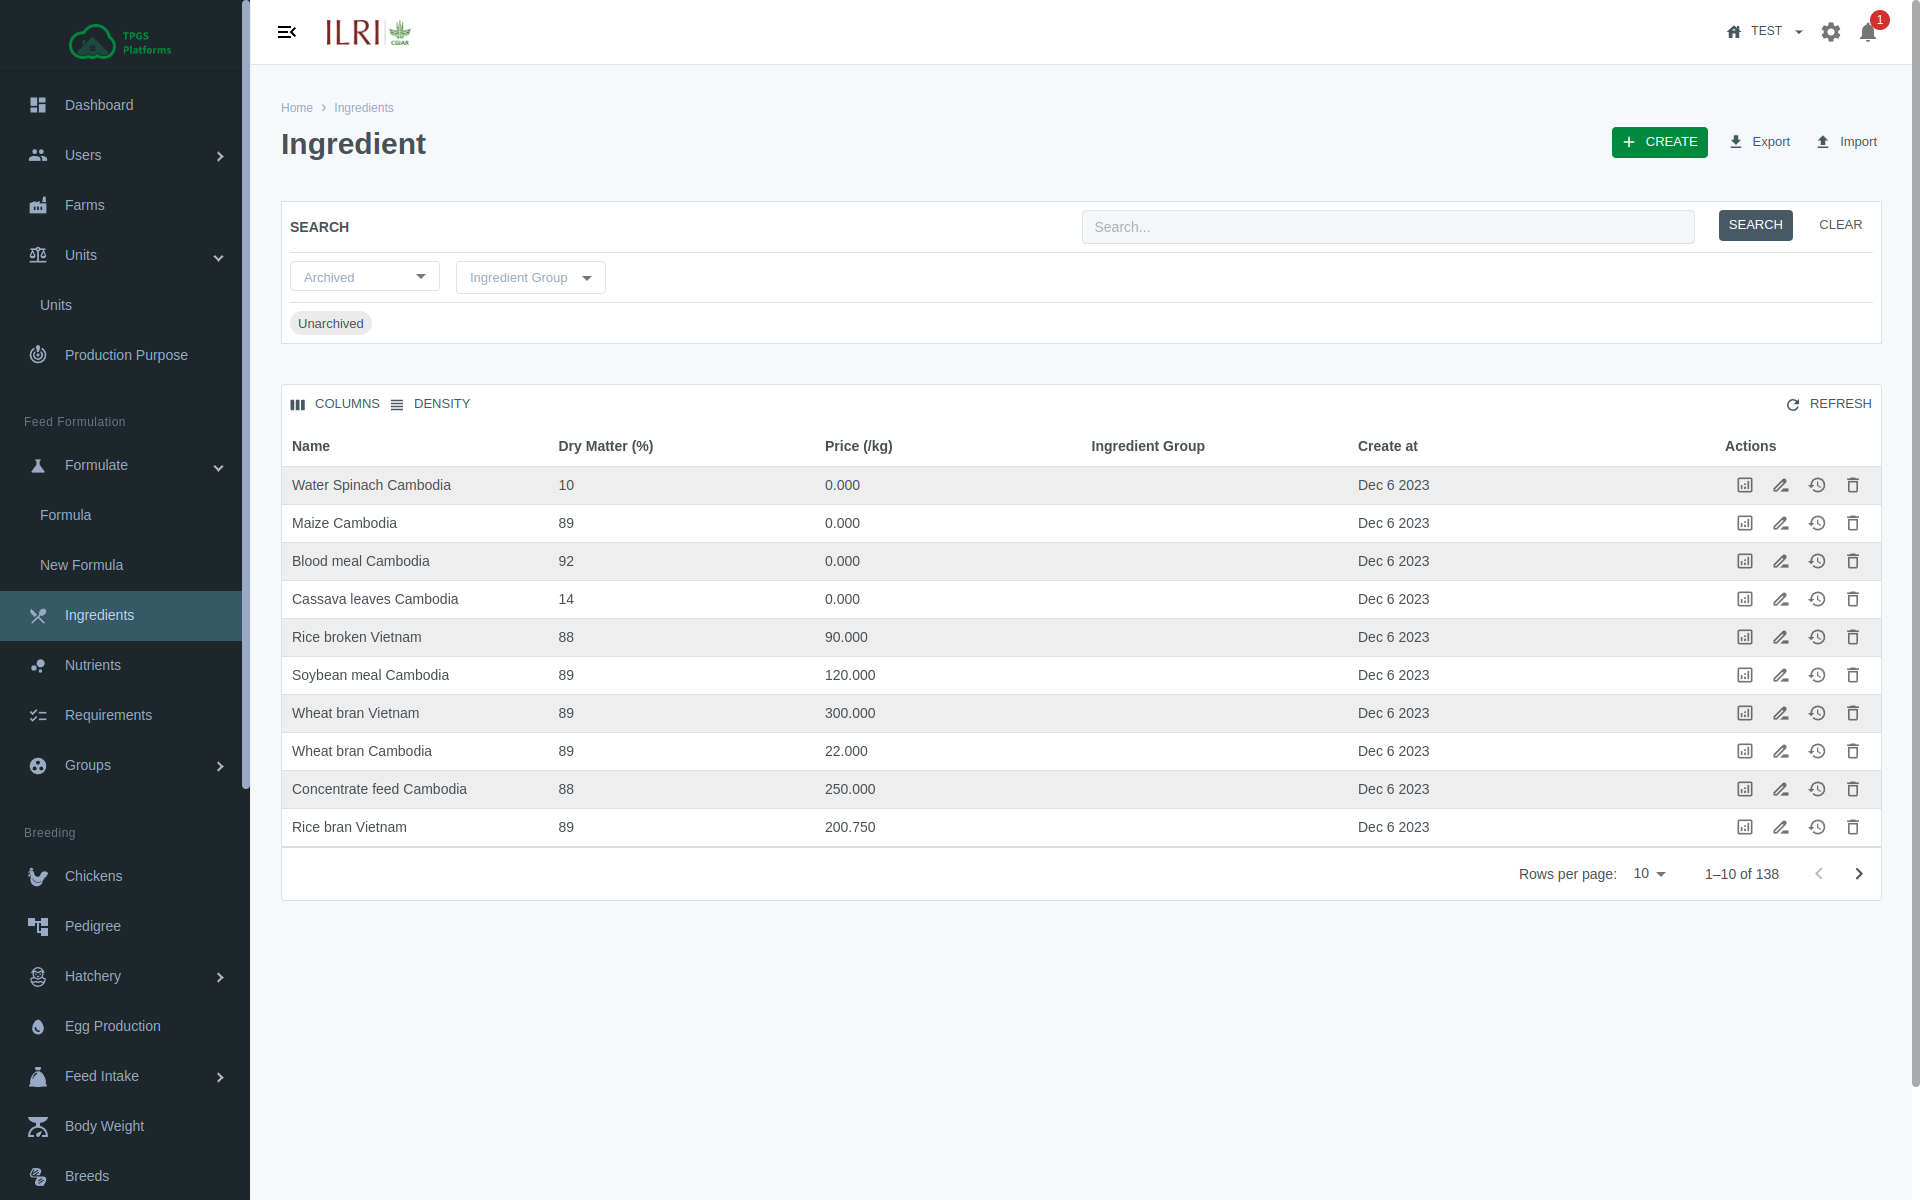
\includegraphics[width=15cm]{s/ingredient_list_page.png}
  	\caption{Ingredients  List}
  	\label{fig:nutrient_list_page}
\end{figure}

\subsection{Archive Records}\label{sec:nutrient_list_archived}
\setcounter{stepcounter}{1}
\paragraph{\arabic{stepcounter}.}On filter section filter the records by archive.

\subsection{Create new Nutrient }\label{sec:nutrient_create}
\setcounter{stepcounter}{1}
\paragraph{\arabic{stepcounter}.}To create new nutrient group click on \textcolor{ForestGreen}{"Create"} \hyperref[fig:nutrient_list_page]{Refer from nutrient list Figure \ref{fig:nutrient_list_page}}
\begin{figure}[h!]
  	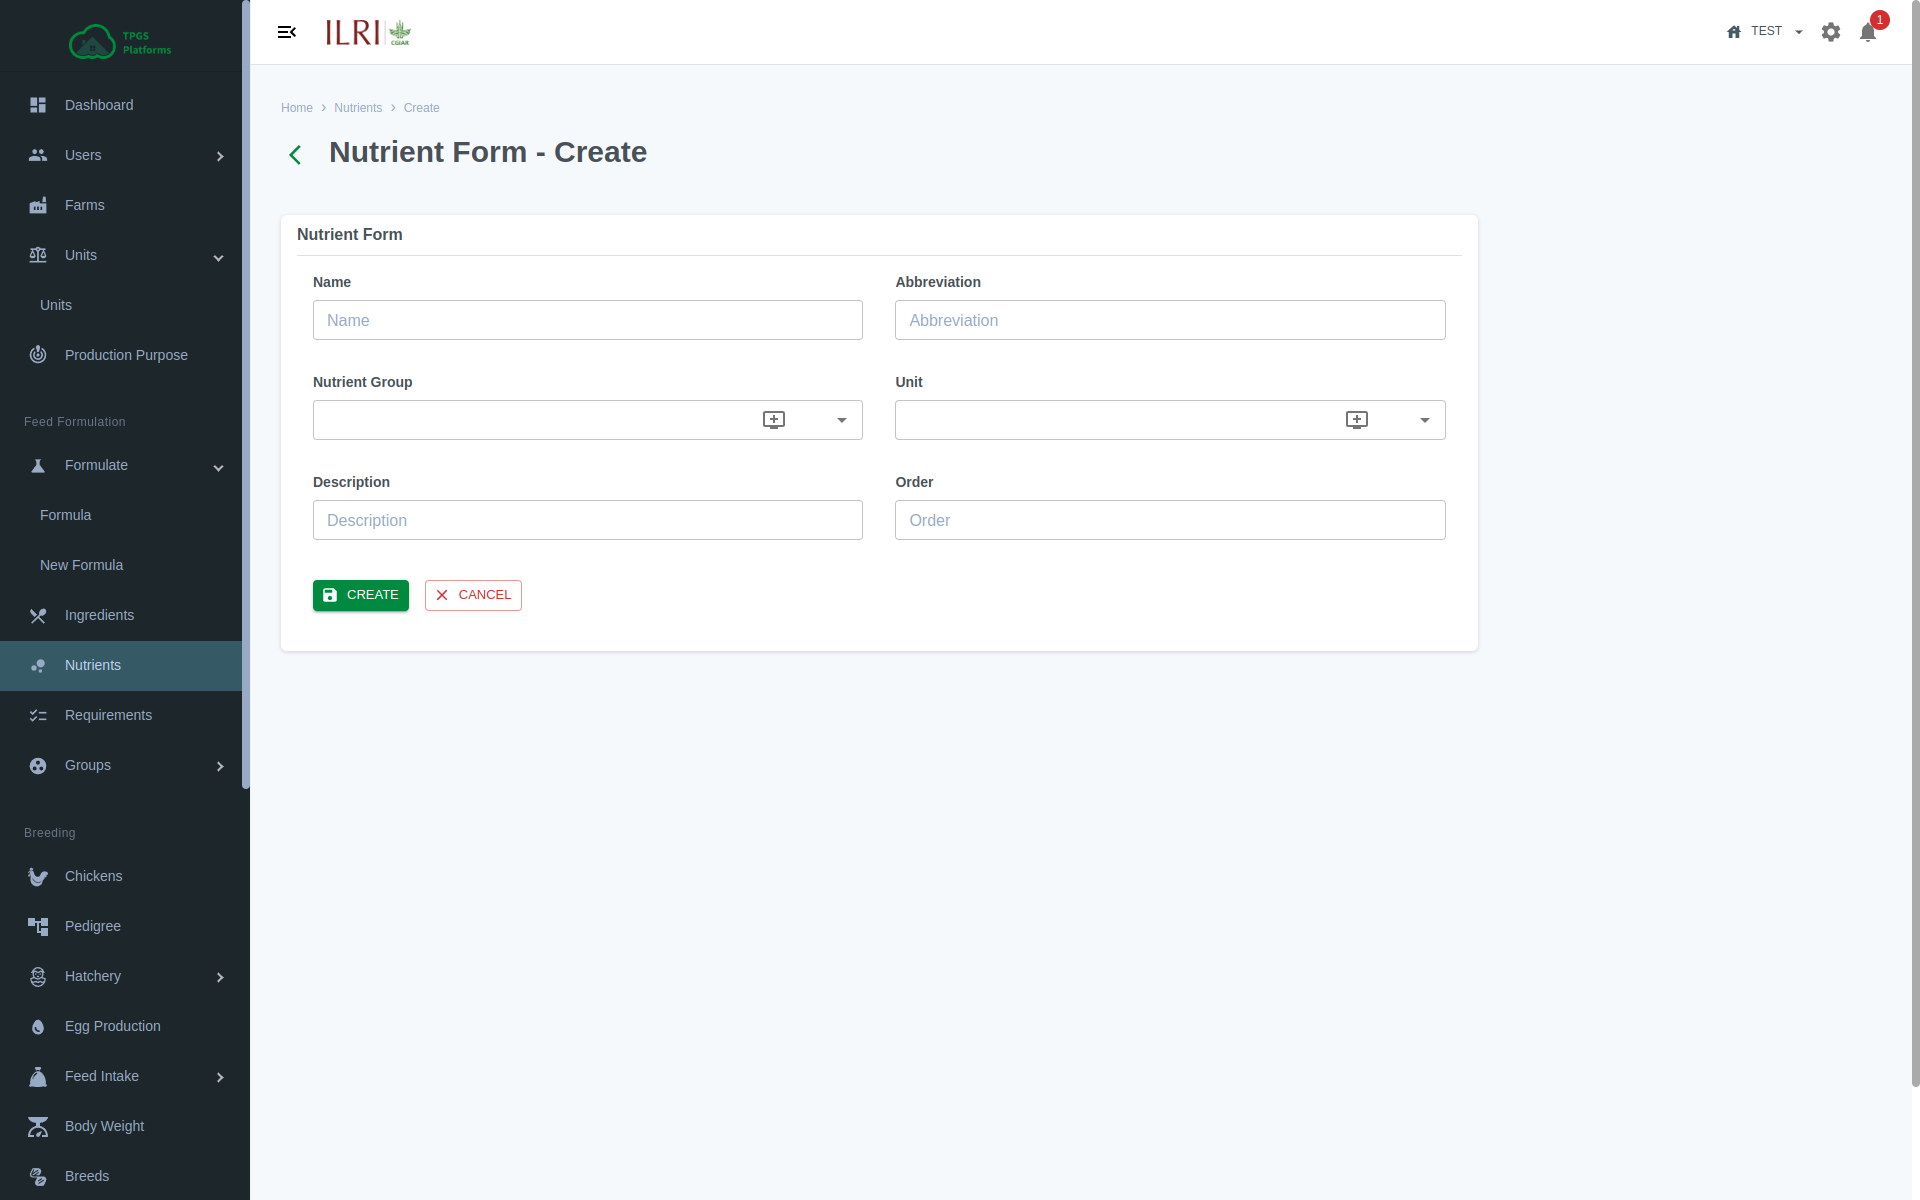
\includegraphics[width=15cm]{screenshots/nutrient_create_page.png}
  	\caption{Create new Nutrient }
  	\label{fig:nutrient_create_page}
\end{figure}
And click \textcolor{ForestGreen}{"CREATE"}, you will be redirect to  \hyperref[sec:nutrient_list]{Nutrient List section \ref{sec:nutrient_list}}

\subsection{Edit Nutrient }\label{sec:nutrient_edit}
\setcounter{stepcounter}{1}
\paragraph{\arabic{stepcounter}.}Go to the Nutrient  \hyperref[sec:nutrient_list]{Refer to Section \ref{sec:nutrient_list}}, then click on Pencil icon and it will redirect to the \hyperref[fig:nutrient_edit_page]{Figure \ref{fig:nutrient_edit_page}}.
\begin{figure}[h!]
  	
\includegraphics[width=15cm]{screenshots/nutrient_edit_page.png}
  	\caption{Edit Nutrient }
  	\label{fig:nutrient_edit_page}
\end{figure}

\subsection{Delete Nutrient }
\setcounter{stepcounter}{1}
\paragraph{\arabic{stepcounter}.}Go to the edit Nutrient  \hyperref[sec:nutrient_edit]{Refer to Section \ref{sec:nutrient_edit}}.

\paragraph{\arabic{stepcounter}.}To archive the record click on \textcolor{ForestGreen}{"Archive"}. If you want to bring back the record/unarchive follow the step under \hyperref[sec:nutrient_list_archived]{Section  \ref{sec:nutrient_list_archived}}, and click on \textcolor{ForestGreen}{"UnArchive"}


\paragraph{\arabic{stepcounter}.}To permanently delete the record click on \textcolor{ForestGreen}{"Delete"}.

\begin{figure}[h!]
  	
\includegraphics[width=15cm]{screenshots/nutrient_edit_page.png}
  	\caption{Edit Nutrient }
  	\label{fig:nutrient_edit_page}
\end{figure}

\newpage

\setcounter{stepcounter}{1}

\paragraph{\arabic{stepcounter}.}Access the website refre to \ref{visite_site}.
If you already have an account login by following  \hyperref[sec:login]{section \ref{sec:login}}.

\stepcounter{stepcounter}
\paragraph{\arabic{stepcounter}.} Enter the required information (Full name, Email address \& message), Click "Submit" and wait for email response.
\begin{figure}[h!]
  	
\includegraphics[width=15cm]{screenshots/sign_up_page.png}
  	\caption{Sign up page}
  	\label{fig:sign_up_page}
\end{figure}

\stepcounter{stepcounter}
\paragraph{\arabic{stepcounter}.} Go to your email inbox to create new account.

\begin{myremark}{Haven't recived invitation email?}\label{visite_site}
You will only recive an invitation email address, if the request is approved by admins. For further detail contact support \hyperref[sec:login]{support address \ref{sec:login}}
\end{myremark}

Click "Join" and you will be redirect to account creation page.
\begin{figure}[h!]
  	
\includegraphics[width=15cm]{screenshots/verify_invitation_page.png}
  	\caption{Verify Invitation Page}
  	\label{fig:verify_invitation_page}
\end{figure}
Enter the required fields and click \textcolor{ForestGreen}{"CREATE NEW ACCOUNT"}.

\newpage
\section{Login}\label{sec:login}
\begin{figure}[h!]
  	
\includegraphics[width=15cm]{screenshots/login_page.png}
  	\caption{Login Page}
  	\label{fig:login_page}
\end{figure}

\newpage
\section{Forgot Password}
There are two ways you can reset your password, you can use  \textcolor{ForestGreen}{"Group"}
\begin{figure}[h!]
  	
\includegraphics[width=15cm]{screenshots/forgot_password_page.png}
  	\caption{Forgot Password Page}
  	\label{fig:forgot_password_page}
\end{figure}

\subsection{Reset password before logged in}ss\begin{equation}
\end{equation}

\subsection{Reset password after logged in}

\newpage
\section{First View}\label{sec:first_view}
\begin{figure}[h!]
  	
\includegraphics[width=15cm]{screenshots/dashboard_page.png}
  	\caption{Dashboard Page}
  	\label{fig:dashboard_page}
\end{figure}

\newpage
\section{Manage Farm}\label{sec:farm}
Switch farm either by going to \textcolor{ForestGreen}{Farms} menu or by click on top right farm menu.
\begin{figure}[h!]
  	
\includegraphics[width=15cm]{screenshots/farm_page.png}
  	\caption{Switch Farm}
  	\label{fig:farm_page}
\end{figure}

\newpage
\section{How to formulate a ration}
\subsection{View Nutrient  List}\label{sec:nutrient_list}
\setcounter{stepcounter}{1}
\paragraph{\arabic{stepcounter}.}On left sidebar menu click \textcolor{ForestGreen}{"Formulate"} then select \textcolor{ForestGreen}{"New Formula"} menu, then you will be redirect to Ration Formulation page.

\begin{figure}[h!]
  	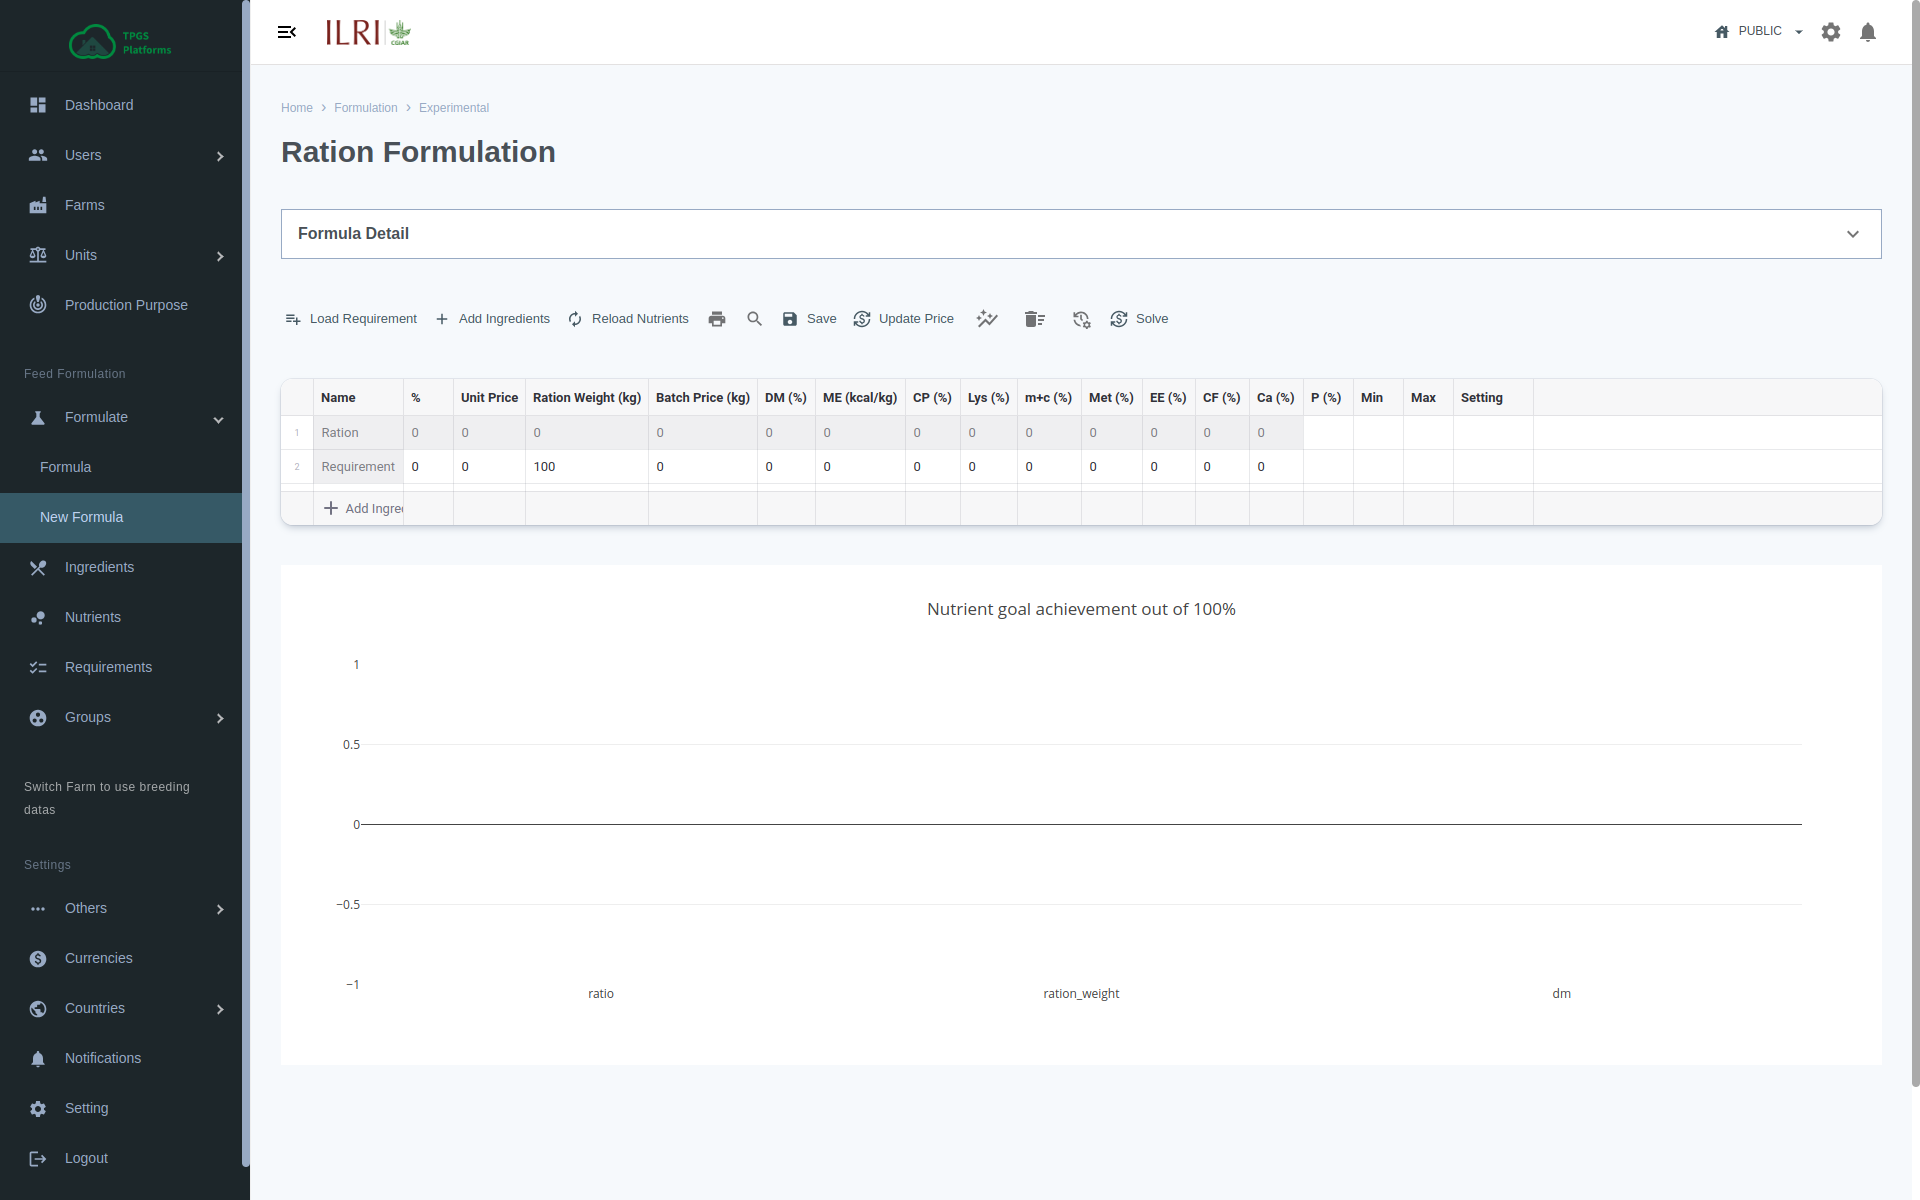
\includegraphics[width=15cm]{screenshots/ration_formulation_page.png}
  	\caption{Ration Formulation page}
  	\label{fig:ration_formulation_page}
\end{figure}

\paragraph{\arabic{stepcounter}.} Select the type of ration you want to prepare by clicking on \textcolor{ForestGreen}{"Load Requirement"}

\begin{figure}[h!]
  	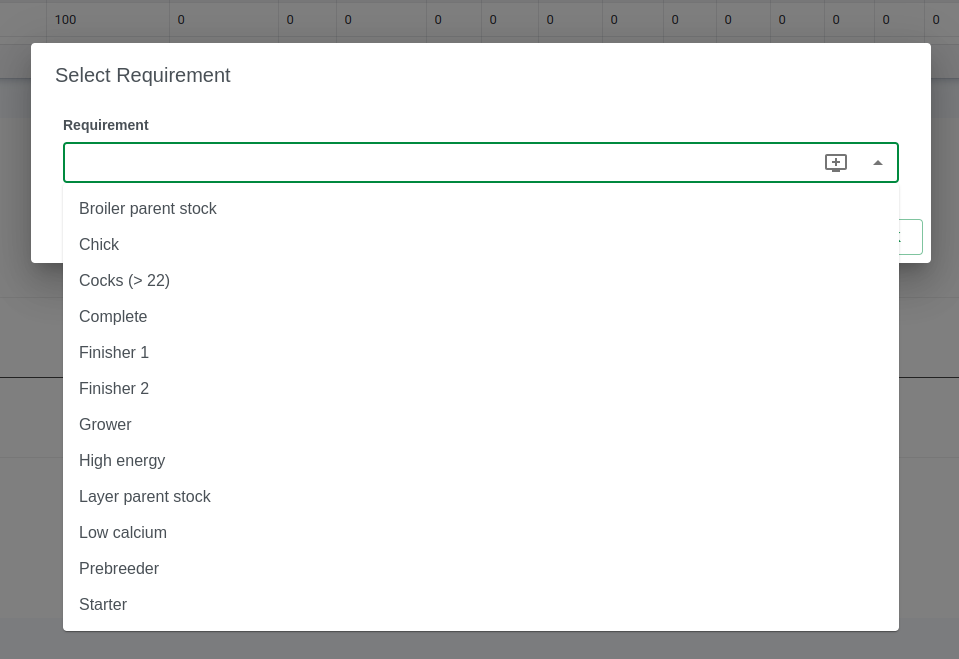
\includegraphics[width=15cm]{screenshots/load_requirement.png}
  	\caption{Load Requirement}
  	\label{fig:load_req}
\end{figure}

\paragraph{\arabic{stepcounter}.} Click \textcolor{ForestGreen}{"Add Ingredients"} to include the required ingredients.

\begin{figure}[h!]
  	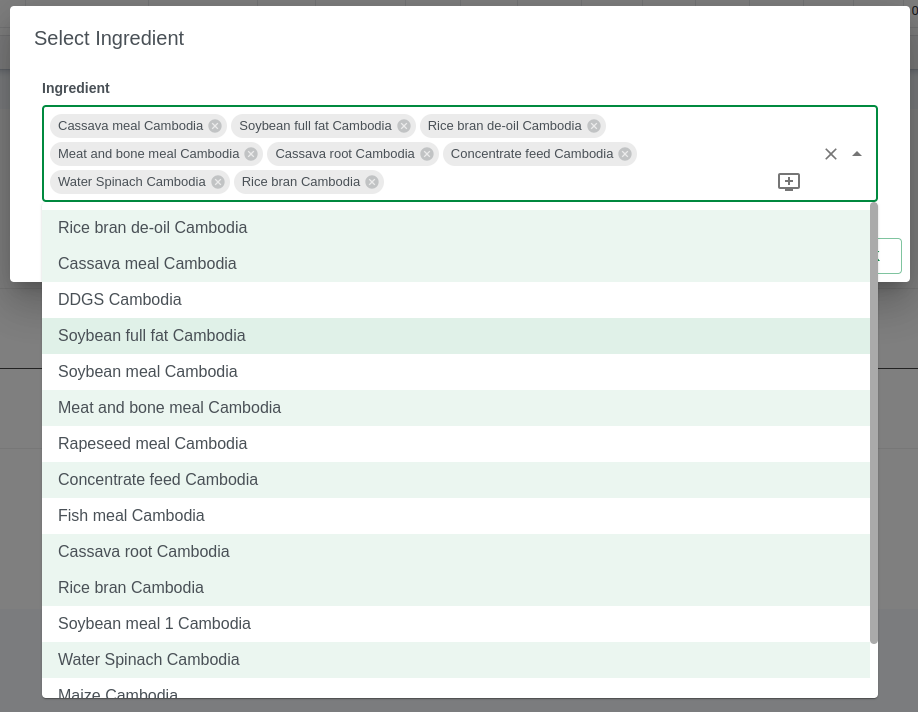
\includegraphics[width=15cm]{screenshots/select_ingredients.png}
  	\caption{Select multiple ingredients}
  	\label{fig:select_ing}
\end{figure}

\paragraph{\arabic{stepcounter}.} If the ingredient you want to include in you ration is not available Refere to \ref{sec:ingredient_create} 

\paragraph{\arabic{stepcounter}.}Formulate your ration ingredient type - \% per 100 kg, price (current price)

\paragraph{\arabic{stepcounter}.} Print or save (to keep it as an archive)

\paragraph{\arabic{stepcounter}.} To update the ingredients with the current price click “Update price”

Remark: If you want to do further analysis on formulated ration click the graph icon

\newpage
\section{Unit}\label{sec:unit}

\subsection{View Unit List}\label{sec:unit_list}
\setcounter{stepcounter}{1}
\paragraph{\arabic{stepcounter}.}Click on \textcolor{ForestGreen}{"Unit"}
\begin{figure}[h!]
  	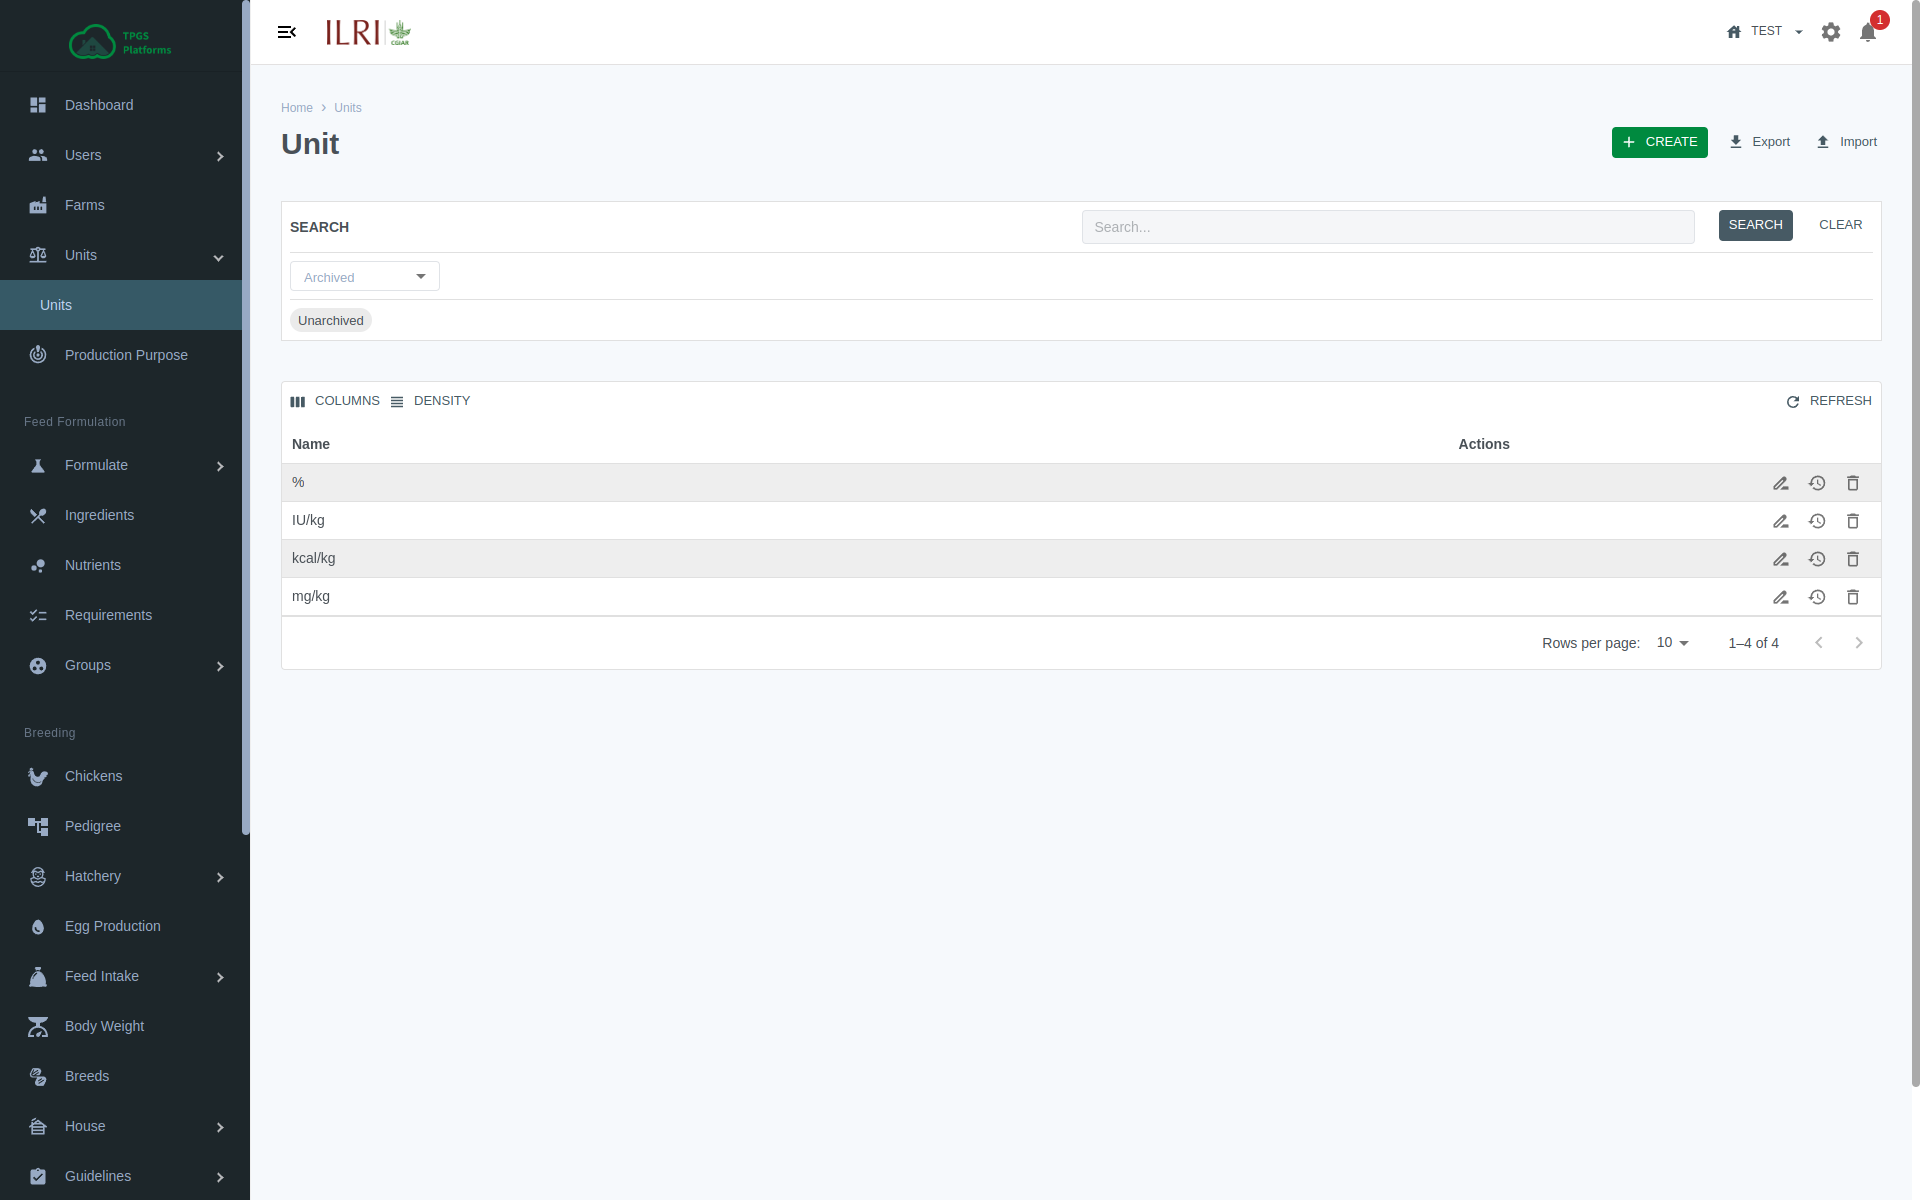
\includegraphics[width=15cm]{screenshots/unit_list_page.png}
  	\caption{Unit List}
  	\label{fig:unit_list_page}
\end{figure}

\subsection{Archive Records}\label{sec:unit_list_archived}
\setcounter{stepcounter}{1}
\paragraph{\arabic{stepcounter}.}On filter section filter the records by archive.

\subsection{Create new Unit}\label{sec:unit_create}
\setcounter{stepcounter}{1}
\paragraph{\arabic{stepcounter}.}To create new unit click on \textcolor{ForestGreen}{"Create"} Refer \hyperref[fig:unit_list_page]{Figure \ref{fig:unit_list_page}}
\begin{figure}[h!]
  	
\includegraphics[width=15cm]{screenshots/unit_create_page.png}
  	\caption{Create new Nutrient Group}
  	\label{fig:unit_create_page}
\end{figure}
And click \textcolor{ForestGreen}{"CREATE"}, you will be redirect to  \hyperref[sec:unit_list]{Section \ref{sec:unit_list}}

\subsection{Edit Unit}\label{sec:unit_edit}
\setcounter{stepcounter}{1}
\paragraph{\arabic{stepcounter}.}Go to the Unit\hyperref[sec:unit_list]{Refer to Section \ref{sec:unit_list}}, then click on Pencil icon and it will redirect to the \hyperref[fig:unit_edit_page]{Figure \ref{fig:unit_edit_page}}.
\begin{figure}[h!]
  	
\includegraphics[width=15cm]{screenshots/unit_edit_page.png}
  	\caption{Edit Unit}
  	\label{fig:unit_edit_page}
\end{figure}

\subsection{Delete Unit}
\setcounter{stepcounter}{1}
\paragraph{\arabic{stepcounter}.}Go to the edit Unit \hyperref[sec:unit_edit]{Refer to Section \ref{sec:unit_edit}}.

\paragraph{\arabic{stepcounter}.}To archive the record click on \textcolor{ForestGreen}{"Archive"}. If you want to bring back the record/unarchive follow the step under \hyperref[sec:unit_list_archived]{Section  \ref{sec:unit_list_archived}}, and click on \textcolor{ForestGreen}{"UnArchive"}


\paragraph{\arabic{stepcounter}.}To permanently delete the record click on \textcolor{ForestGreen}{"Delete"}.

\begin{figure}[h!]
  	
\includegraphics[width=15cm]{screenshots/unit_edit_page.png}
  	\caption{Edit Unit}
  	\label{fig:unit_edit_page}
\end{figure}

\newpage
%\section{Production Purposes}\label{sec:production_purpose}

\subsection{Production Purpose List}\label{sec:production_purpose_list}
\setcounter{stepcounter}{1}
\paragraph{\arabic{stepcounter}.}Access Production Purposes list by clicking on \textcolor{ForestGreen}{"Production Purpose"} from left 
\paragraph{\arabic{stepcounter}.}Expand \textcolor{ForestGreen}{"Group"} menu and click on \textcolor{ForestGreen}{"Nutrient Group"}
\begin{figure}[h!]
  	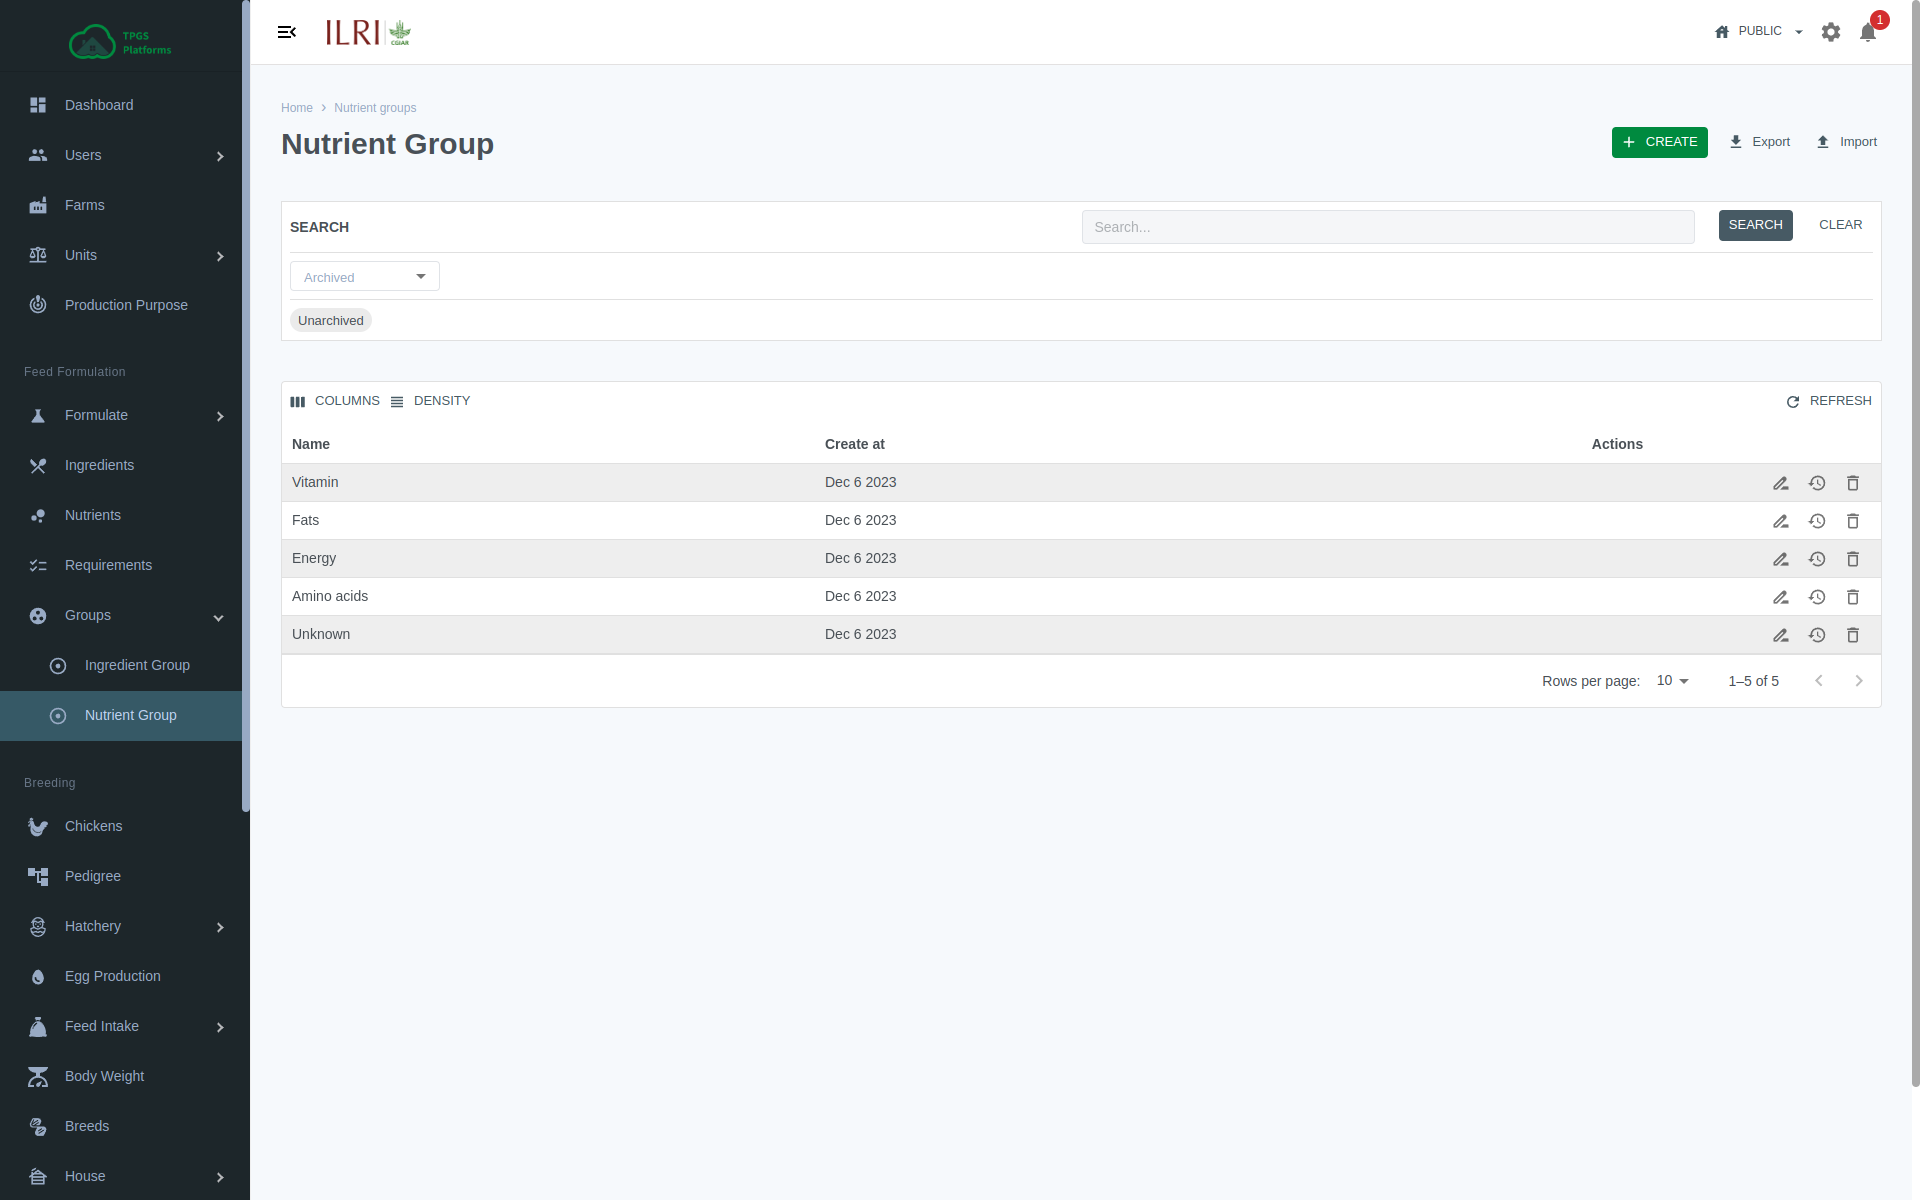
\includegraphics[width=15cm]{screenshots/nutrient_group_list_page.png}
  	\caption{Nutrient Group List}
  	\label{fig:nutrient_group_list_page}
\end{figure}

\subsection{Archive Records}\label{sec:nutrient_group_list_archived}
\setcounter{stepcounter}{1}
\paragraph{\arabic{stepcounter}.}On filter section filter the records by archive.

\subsection{Create new Nutrient Group}\label{sec:nutrient_group_create}
\setcounter{stepcounter}{1}
\paragraph{\arabic{stepcounter}.}To create new nutrient group click on \textcolor{ForestGreen}{"Create"} \hyperref[fig:nutrient_group_list_page]{Refer from nutrient list Figure \ref{fig:nutrient_group_list_page}}
\begin{figure}[h!]
  	
\includegraphics[width=15cm]{screenshots/nutrient_group_create_page.png}
  	\caption{Create new Nutrient Group}
  	\label{fig:nutrient_group_create_page}
\end{figure}
And click \textcolor{ForestGreen}{"CREATE"}, you will be redirect to  \hyperref[sec:nutrient_group_list]{Nutrient List section \ref{sec:nutrient_group_list}}

\subsection{Edit Nutrient Group}\label{sec:nutrient_group_edit}
\setcounter{stepcounter}{1}
\paragraph{\arabic{stepcounter}.}Go to the Nutrient Group \hyperref[sec:nutrient_group_list]{Refer to Section \ref{sec:nutrient_group_list}}, then click on Pencil icon and it will redirect to the \hyperref[fig:nutrient_group_edit_page]{Figure \ref{fig:nutrient_group_edit_page}}.
\begin{figure}[h!]
  	
\includegraphics[width=15cm]{screenshots/nutrient_group_edit_page.png}
  	\caption{Edit Nutrient Group}
  	\label{fig:nutrient_group_edit_page}
\end{figure}

\subsection{Delete Nutrient Group}
\setcounter{stepcounter}{1}
\paragraph{\arabic{stepcounter}.}Go to the edit Nutrient Group \hyperref[sec:nutrient_group_edit]{Refer to Section \ref{sec:nutrient_group_edit}}.

\paragraph{\arabic{stepcounter}.}To archive the record click on \textcolor{ForestGreen}{"Archive"}. If you want to bring back the record/unarchive follow the step under \hyperref[sec:nutrient_group_list_archived]{Section  \ref{sec:nutrient_group_list_archived}}, and click on \textcolor{ForestGreen}{"UnArchive"}


\paragraph{\arabic{stepcounter}.}To permanently delete the record click on \textcolor{ForestGreen}{"Delete"}.

\begin{figure}[h!]
  	
\includegraphics[width=15cm]{screenshots/nutrient_group_edit_page.png}
  	\caption{Edit Nutrient Group}
  	\label{fig:nutrient_group_edit_page}
\end{figure}

%\section{Invitation}

%\subsection{View Invitations List}
%\subsection{Invite User}
%\subsection{Resend Invitation}
%\subsection{Remove Invitation}

%\section{Users}

%\subsection{View Users List}
%\subsection{Edit User}
%\subsection{Deactivate/Activate User's Account}
%\subsection{Delete User}

%\section{Settings}
%\subsection{Change Password}


\newpage
\section{Nutrient Groups}\label{sec:nutrient_group}

\subsection{View Nutrient Group List}\label{sec:nutrient_group_list}
\setcounter{stepcounter}{1}
\paragraph{\arabic{stepcounter}.}Expand \textcolor{ForestGreen}{"Group"} menu and click on \textcolor{ForestGreen}{"Nutrient Group"}
\begin{figure}[h!]
  	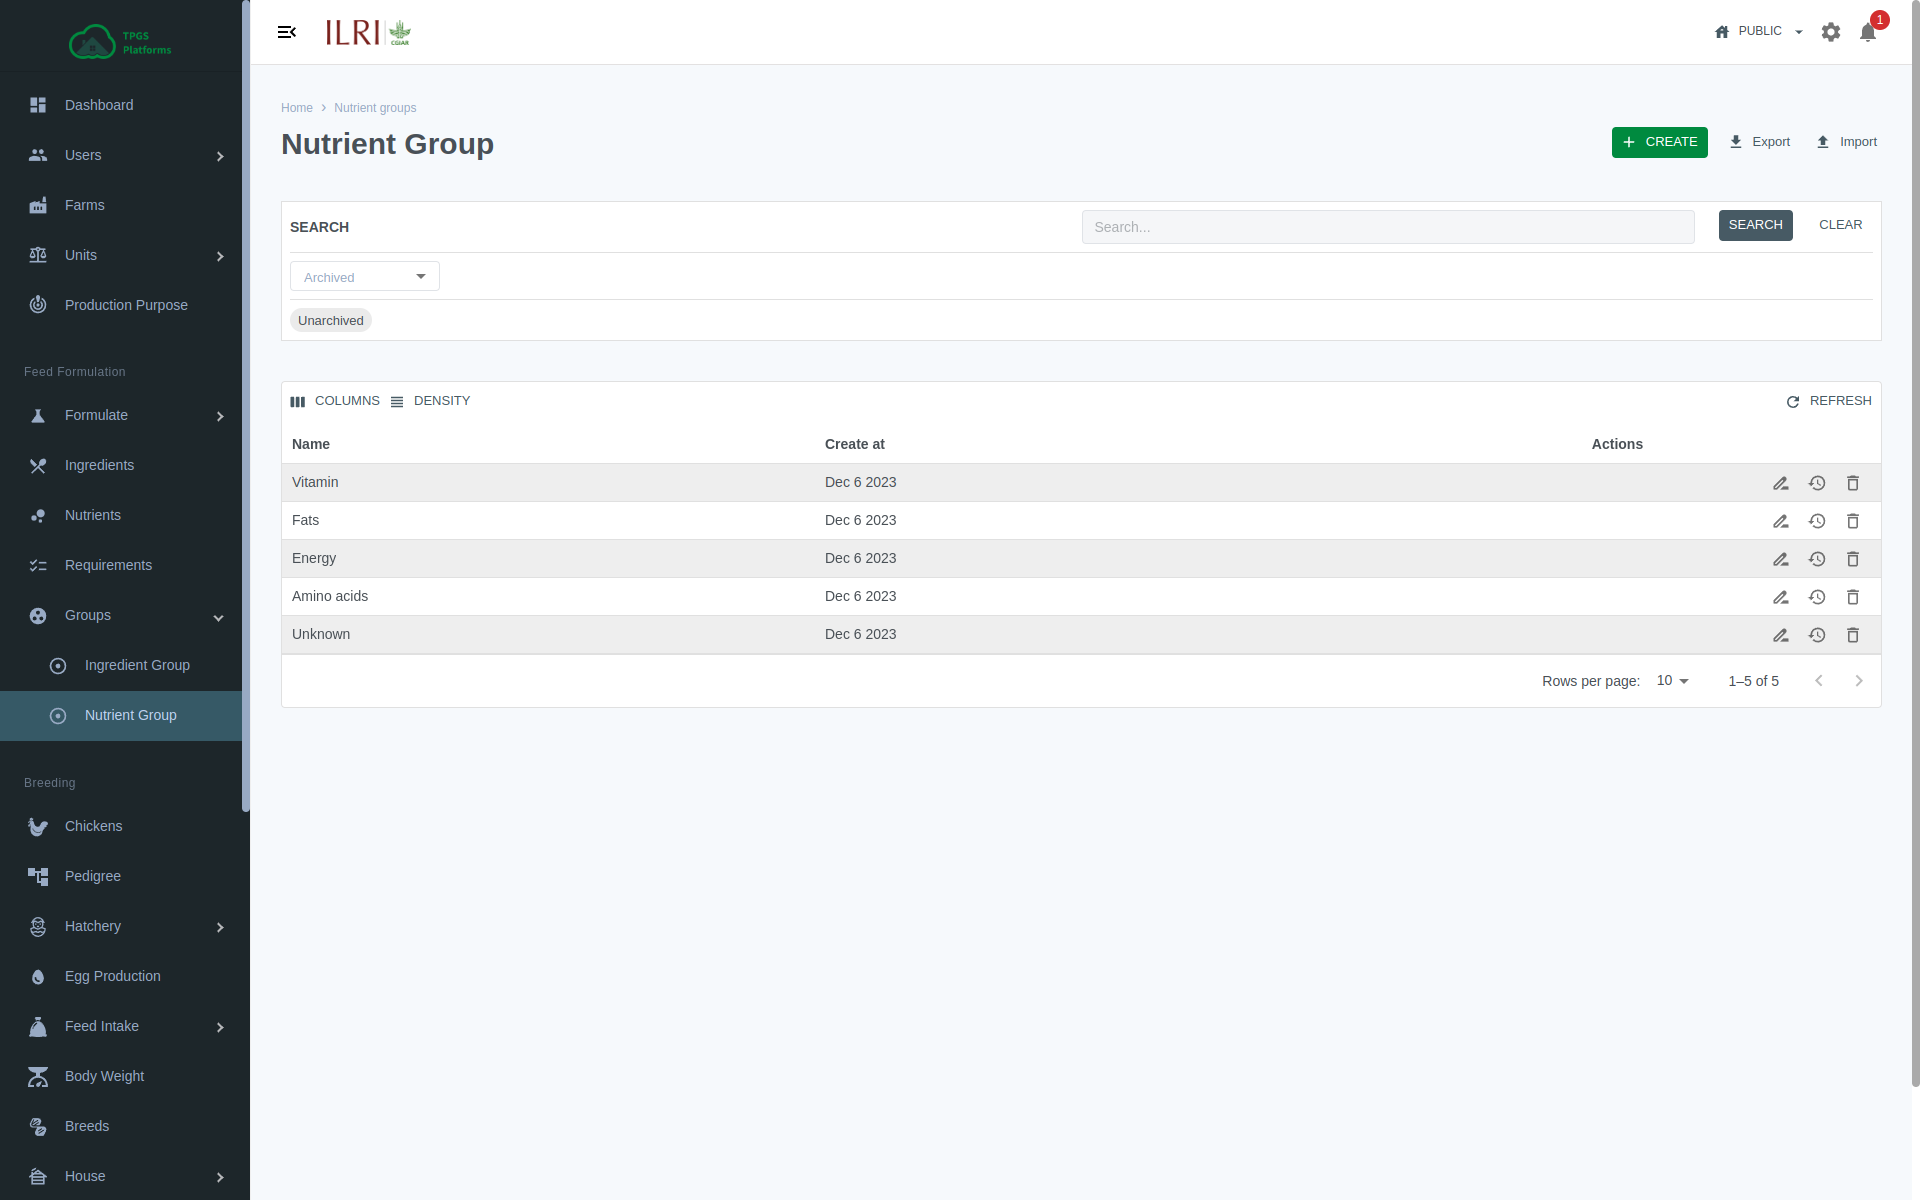
\includegraphics[width=15cm]{screenshots/nutrient_group_list_page.png}
  	\caption{Nutrient Group List}
  	\label{fig:nutrient_group_list_page}
\end{figure}

\subsection{Archive Records}\label{sec:nutrient_group_list_archived}
\setcounter{stepcounter}{1}
\paragraph{\arabic{stepcounter}.}On filter section filter the records by archive.

\subsection{Create new Nutrient Group}\label{sec:nutrient_group_create}
\setcounter{stepcounter}{1}
\paragraph{\arabic{stepcounter}.}To create new nutrient group click on \textcolor{ForestGreen}{"Create"} \hyperref[fig:nutrient_group_list_page]{Refer from nutrient list Figure \ref{fig:nutrient_group_list_page}}
\begin{figure}[h!]
  	
\includegraphics[width=15cm]{screenshots/nutrient_group_create_page.png}
  	\caption{Create new Nutrient Group}
  	\label{fig:nutrient_group_create_page}
\end{figure}
And click \textcolor{ForestGreen}{"CREATE"}, you will be redirect to  \hyperref[sec:nutrient_group_list]{Nutrient List section \ref{sec:nutrient_group_list}}

\subsection{Edit Nutrient Group}\label{sec:nutrient_group_edit}
\setcounter{stepcounter}{1}
\paragraph{\arabic{stepcounter}.}Go to the Nutrient Group \hyperref[sec:nutrient_group_list]{Refer to Section \ref{sec:nutrient_group_list}}, then click on Pencil icon and it will redirect to the \hyperref[fig:nutrient_group_edit_page]{Figure \ref{fig:nutrient_group_edit_page}}.
\begin{figure}[h!]
  	
\includegraphics[width=15cm]{screenshots/nutrient_group_edit_page.png}
  	\caption{Edit Nutrient Group}
  	\label{fig:nutrient_group_edit_page}
\end{figure}

\subsection{Delete Nutrient Group}
\setcounter{stepcounter}{1}
\paragraph{\arabic{stepcounter}.}Go to the edit Nutrient Group \hyperref[sec:nutrient_group_edit]{Refer to Section \ref{sec:nutrient_group_edit}}.

\paragraph{\arabic{stepcounter}.}To archive the record click on \textcolor{ForestGreen}{"Archive"}. If you want to bring back the record/unarchive follow the step under \hyperref[sec:nutrient_group_list_archived]{Section  \ref{sec:nutrient_group_list_archived}}, and click on \textcolor{ForestGreen}{"UnArchive"}


\paragraph{\arabic{stepcounter}.}To permanently delete the record click on \textcolor{ForestGreen}{"Delete"}.

\begin{figure}[h!]
  	
\includegraphics[width=15cm]{screenshots/nutrient_group_edit_page.png}
  	\caption{Edit Nutrient Group}
  	\label{fig:nutrient_group_edit_page}
\end{figure}

\newpage
\section{Nutrient}\label{sec:nutrient}

\subsection{View Nutrient  List}\label{sec:nutrient_list}
\setcounter{stepcounter}{1}
\paragraph{\arabic{stepcounter}.}Expand \textcolor{ForestGreen}{"Group"} menu and click on \textcolor{ForestGreen}{"Nutrient "}
\begin{figure}[h!]
  	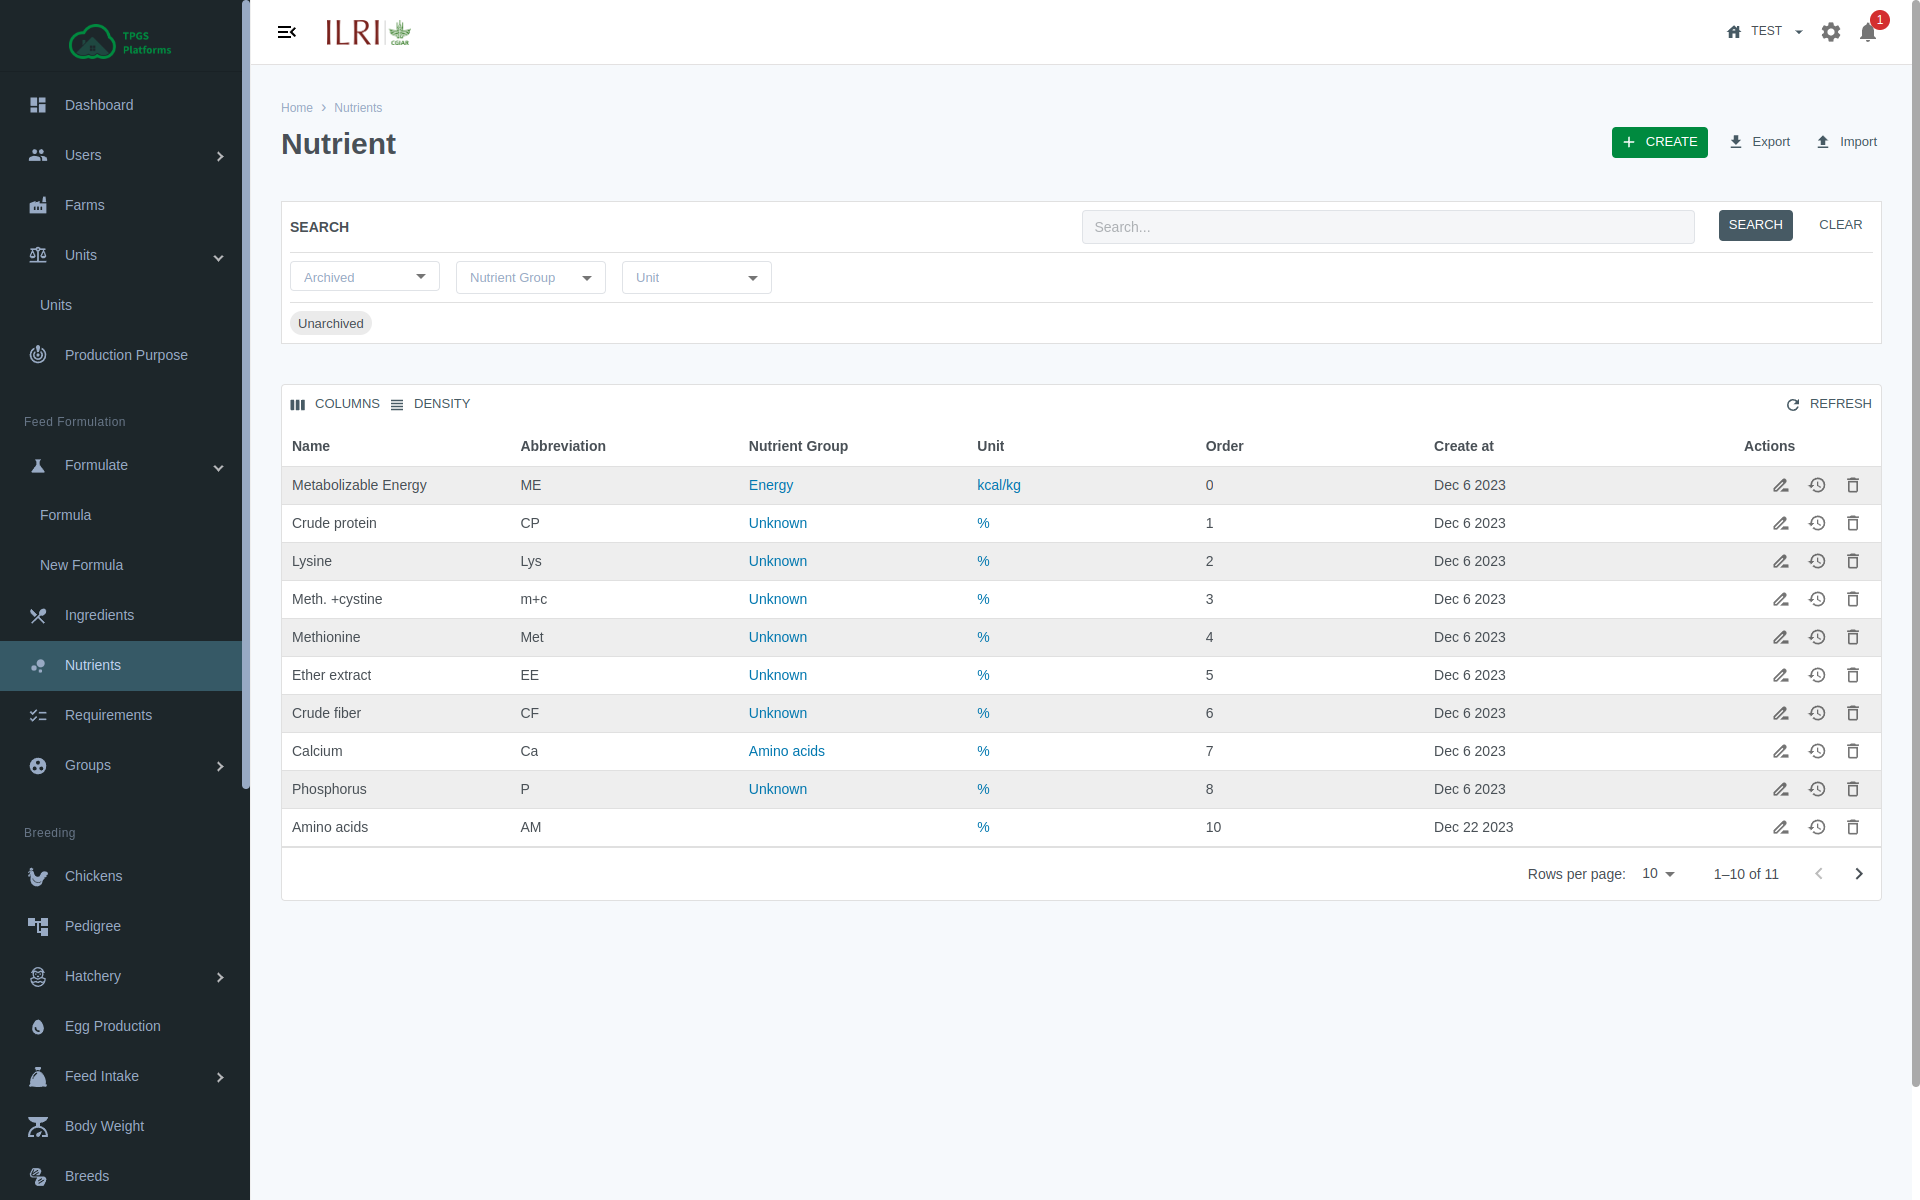
\includegraphics[width=15cm]{screenshots/nutrient_list_page.png}
  	\caption{Nutrient  List}
  	\label{fig:nutrient_list_page}
\end{figure}

\subsection{Archive Records}\label{sec:nutrient_list_archived}
\setcounter{stepcounter}{1}
\paragraph{\arabic{stepcounter}.}On filter section filter the records by archive.

\subsection{Create new Nutrient }\label{sec:nutrient_create}
\setcounter{stepcounter}{1}
\paragraph{\arabic{stepcounter}.}To create new nutrient group click on \textcolor{ForestGreen}{"Create"} \hyperref[fig:nutrient_list_page]{Refer from nutrient list Figure \ref{fig:nutrient_list_page}}
\begin{figure}[h!]
  	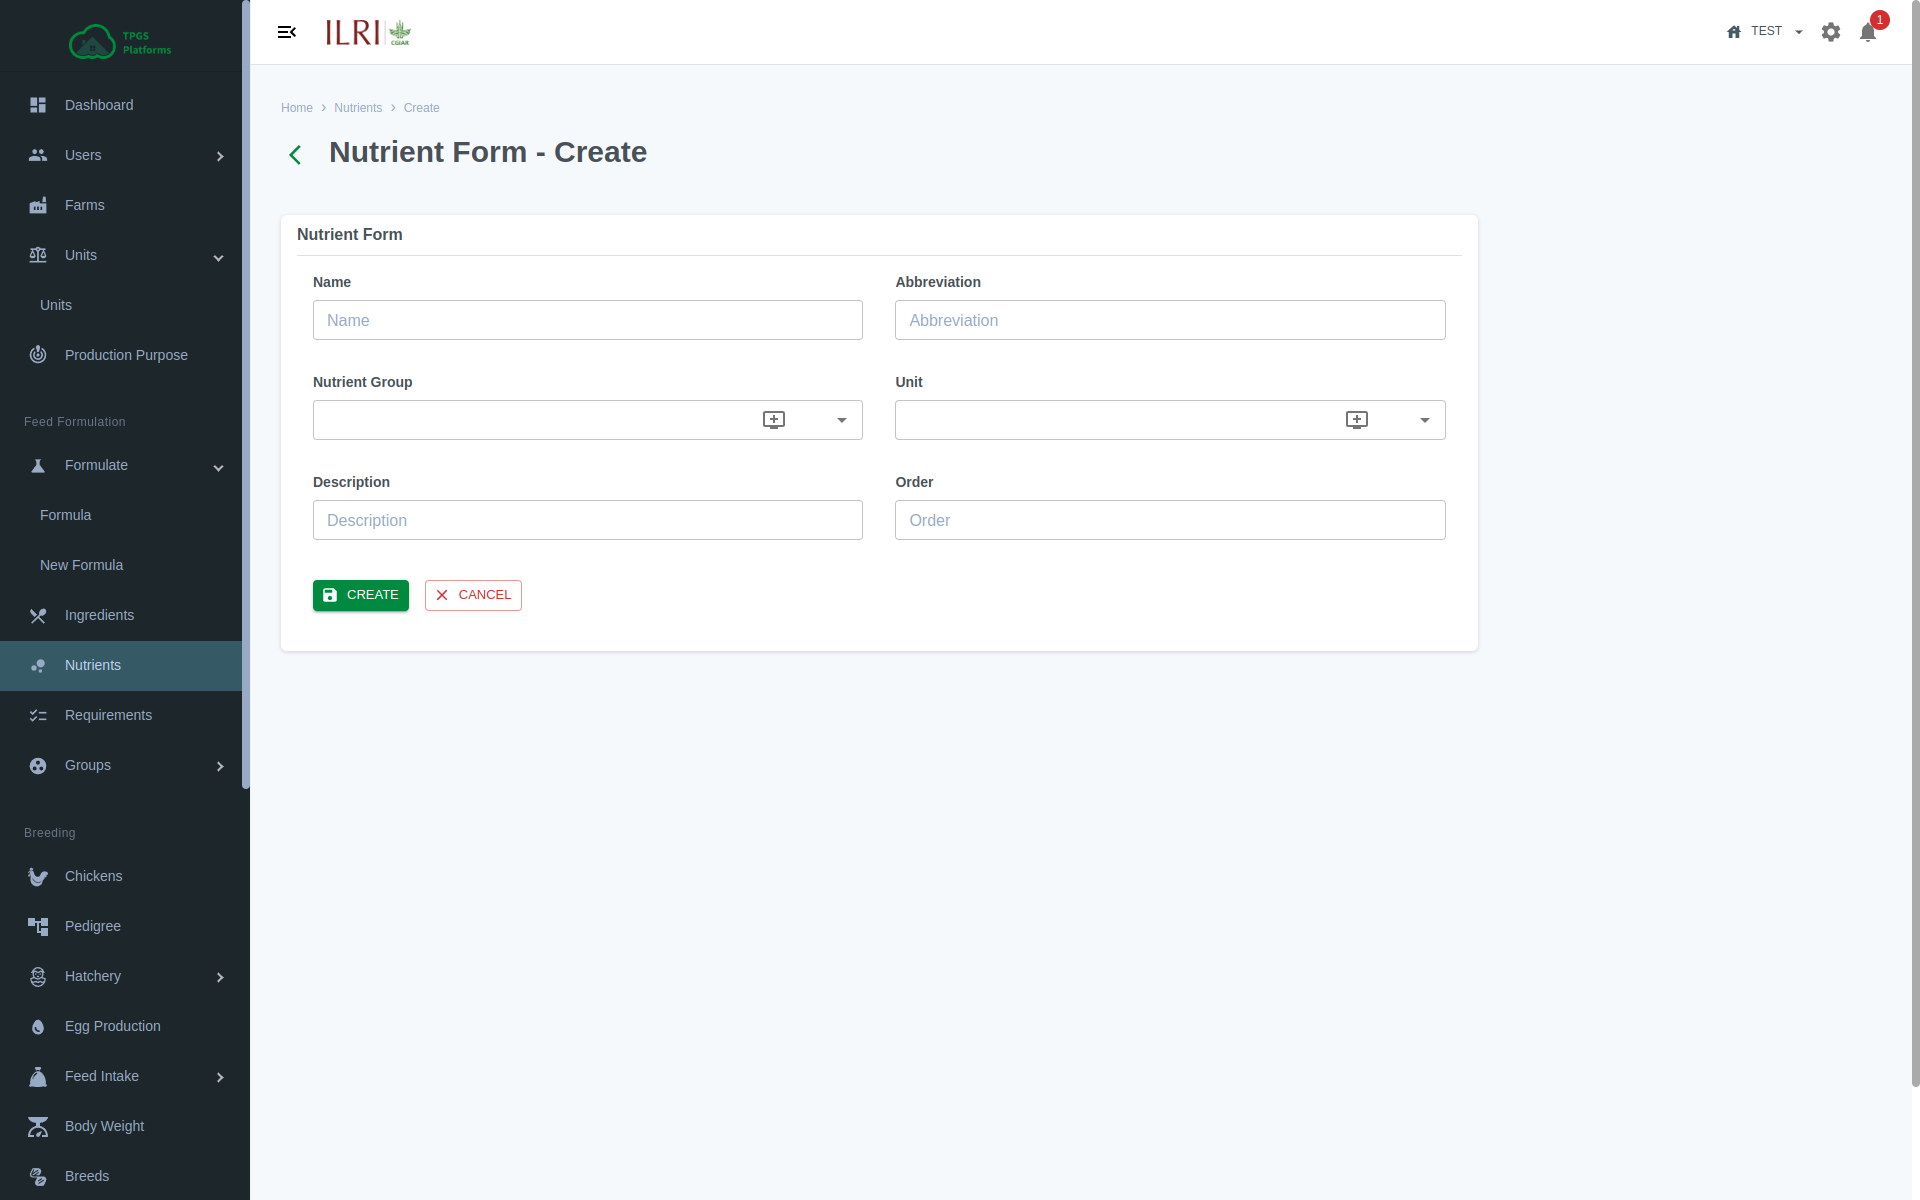
\includegraphics[width=15cm]{screenshots/nutrient_create_page.png}
  	\caption{Create new Nutrient }
  	\label{fig:nutrient_create_page}
\end{figure}
And click \textcolor{ForestGreen}{"CREATE"}, you will be redirect to  \hyperref[sec:nutrient_list]{Nutrient List section \ref{sec:nutrient_list}}

\subsection{Edit Nutrient }\label{sec:nutrient_edit}
\setcounter{stepcounter}{1}
\paragraph{\arabic{stepcounter}.}Go to the Nutrient  \hyperref[sec:nutrient_list]{Refer to Section \ref{sec:nutrient_list}}, then click on Pencil icon and it will redirect to the \hyperref[fig:nutrient_edit_page]{Figure \ref{fig:nutrient_edit_page}}.
\begin{figure}[h!]
  	
\includegraphics[width=15cm]{screenshots/nutrient_edit_page.png}
  	\caption{Edit Nutrient }
  	\label{fig:nutrient_edit_page}
\end{figure}

\subsection{Delete Nutrient }
\setcounter{stepcounter}{1}
\paragraph{\arabic{stepcounter}.}Go to the edit Nutrient  \hyperref[sec:nutrient_edit]{Refer to Section \ref{sec:nutrient_edit}}.

\paragraph{\arabic{stepcounter}.}To archive the record click on \textcolor{ForestGreen}{"Archive"}. If you want to bring back the record/unarchive follow the step under \hyperref[sec:nutrient_list_archived]{Section  \ref{sec:nutrient_list_archived}}, and click on \textcolor{ForestGreen}{"UnArchive"}


\paragraph{\arabic{stepcounter}.}To permanently delete the record click on \textcolor{ForestGreen}{"Delete"}.

\begin{figure}[h!]
  	
\includegraphics[width=15cm]{screenshots/nutrient_edit_page.png}
  	\caption{Edit Nutrient }
  	\label{fig:nutrient_edit_page}
\end{figure}

%\section{Ration Formulation}


\newpage
\section{Contact Info}\label{sec:contact_info}

For further information contact W.Esatu@cgiar.org

\newpage
\section{Reference}
%\nocite{*}
%\printbibliography


\begin{enumerate}
	\item De Blas, C., \& Mateos, G. G. (2010). Feed Formulation for Poultry and Other Livestock.
	\item De Blas, C., \& Mateos, G. G. (2010). Feed Formulation for Poultry and Other Livestock. This text covers the formulation of poultry diets, including the role of fats and the need
for antioxidants in maintaining feed quality.

	\item Emmert, J. L., \& Baker, D. H. (1997). "Use of crystalline amino acids in poultry diets: A
review." Journal of Applied Poultry Research, 6(4), 471-480. This review discusses the
use of synthetic amino acids like methionine and lysine in poultry diets and their benefits
in balanced feed formulation.
	
	\item Faria, D. E., \& Faria Filho, D. E. (2020). Poultry Feed Ingredients: Nutritional Value and
Safety.

	\item Gonzalez-Esquerra, R., \& Leeson, S. (2001). "Effects of feeding birds with diets high in
fat and linoleic acid." Poultry Science, 80(8), 1171-1176. This study provides insights into
how dietary fats and linoleic acid affect growth, egg production, and feed efficiency in
poultry.

	\item Leeson, S., \& Summers, J. D. (2001). Nutrition of the Chicken. University Books.
	
	\item Leeson, S., \& Summers, J. D. (2001). Nutrition of the Chicken. University Books. This
book details the importance of essential fatty acids like linoleic acid in poultry nutrition,
emphasizing their role in reproductive health and growth.

	\item Leeson, S., \& Summers, J. D. (2001). Nutrition of the Chicken. University Books. This
text covers protein and amino acid needs for poultry, with a focus on diet formulation and
essential amino acids.

	\item Leeson, S., \& Summers, J. D. (2001). Nutrition of the Chicken. University Books. This
book discusses mineral sources in poultry diets and the roles of both macro- and
microminerals in supporting health and production.

	\item Leeson, S., \& Summers, J. D. (2001). Nutrition of the Chicken. University Books. This
book provides detailed information on the roles and dietary requirements of vitamins in
poultry, including the importance of vitamin premixes.

	\item McDowell, L. R. (2000). Vitamins in Animal Nutrition. Academic Press. This text
discusses the functions, sources, and stability of vitamins in poultry feed, including
natural sources and the need for premixes.

	\item National Research Council (NRC). (1994). Nutrient Requirements of Poultry. National
Academy Press.

	\item National Research Council (NRC). (1994). Nutrient Requirements of Poultry. National
Academy Press. This reference provides essential nutrient requirements for poultry,
including recommended levels of linoleic acid and other fats.

	\item National Research Council (NRC). (1994). Nutrient Requirements of Poultry. National
Academy Press. This source provides nutrient requirements for poultry, including amino
acid profiles and the role of protein sources.

	\item National Research Council (NRC). (1994). Nutrient Requirements of Poultry. National
Academy Press. This reference details the mineral requirements of poultry, including
macromineral and micromineral recommendations.

	\item National Research Council (NRC). (1994). Nutrient Requirements of Poultry. National
Academy Press. This reference outlines the vitamin requirements for poultry and the
importance of supplementation.

	\item Pardue, S. L., \& Thaxton, J. P. (1984). "Ascorbic acid in poultry: A review." Poultry
Science, 63(1), 1767-1776. This review explains the role of vitamin C in poultry,
especially under stress conditions.

	\item Pesti, G. M., \& Bakalli, R. I. (1997). "Studies on the feeding value of low-mineral
supplements in poultry diets." Poultry Science, 76(6), 914-920. This study examines
mineral supplementation in poultry diets and the consequences of inadequate mineral
levels

	\item Ravindran, V., \& Blair, R. (1991). "Feed resources for poultry production in Asia and the
Pacific. "World's Poultry Science Journal, 47(3), 213-231. This study explores the protein
sources available for poultry feed, including fish meal, and highlights concerns regarding
anti-nutritional factors and flavor changes in poultry products.

	\item Underwood, E. J., \& Suttle, N. F. (1999). The Mineral Nutrition of Livestock. This book
provides an in-depth overview of mineral functions, deficiency symptoms, and the
importance of balancing minerals in animal diets, including poultry.

	\item Leeson, S., \& Summers, J. D. (2009). Commercial Poultry Nutrition (4th ed.).
University Books.

	\item Ravindran, V., \& Blair, R. (2013). Poultry Feed and Nutrition (2nd ed.). CAB
International.

	\item Nitray, P., \& Tiwari, R. (2019). Feed formulation and optimization in poultry
farming. International Journal of Poultry Science, 18(1), 11-20.

	\item FAO (2017). Sustainable Poultry Production and Feed Formulation Techniques.
Food and Agriculture Organization of the United Nations.

	
\end{enumerate}

\end{document}